% !TEX program = pdflatex
% ==============================================================================
% BIỂU MẪU BÁO CÁO VÀ BÀI TẬP KHOA CÔNG NGHỆ THÔNG TIN - ĐH KHTN (ĐHQG-HCM)
% Biên dịch bằng: PDFLaTeX
% ==============================================================================
\documentclass[12pt,a4paper]{article}
\usepackage{scrextend}
\changefontsizes{13pt}

% Nạp gói cấu hình chuẩn nhận diện FIT - HCMUS
\usepackage{fit_hcmus}
\setcounter{secnumdepth}{2}
\setcounter{tocdepth}{2}

% ==============================================================================
% KHAI BÁO THÔNG TIN BÀI TẬP / ĐỒ ÁN
% ==============================================================================
\courseid{CSC14003}
\coursename{Cơ Sở Trí Tuệ Nhân Tạo}
\reportsubtitle{BÁO CÁO ĐỒ ÁN MÔN HỌC}
\title{Đồ án Griductive Solver}
\instructor{TS. Bùi Tiến Lên}
\labinstructor{TA. Nguyễn Thanh Tình}
\classid{CQ2024/22}
\academicyear{Học kỳ I, 2026 - 2027}

% Khai báo danh sách sinh viên thực hiện
\author{
    \centering
    \begin{tabular}{ll}
        Ngô Hoàng Minh & - 24120381 \\
        Nguyễn Xuân Lộc & - 24120369 \\
        Đỗ Ngọc Hải & - 24120300 \\
        Nguyễn Thành Bảo & - 24120023 \\
        Phan Nhật Minh & - 24120384 \\
    \end{tabular}
}

% ==============================================================================
% CHỌN CHẾ ĐỘ HIỂN THỊ (PROJECT HOẶC ASSIGNMENT/LAB)
% Đặt true nếu là Báo cáo đồ án (có trang bìa riêng, mục lục)
% Đặt false nếu là Bài tập cá nhân / Lab ngắn gọn (dùng header đầu trang 1)
% ==============================================================================
\newif\ifisprojectreport
\isprojectreporttrue % <--- ĐỔI THÀNH \isprojectreportfalse CHO BÀI TẬP NGẮN

\begin{document}

\ifisprojectreport
    % --- CHẾ ĐỘ 1: BÁO CÁO ĐỒ ÁN MÔN HỌC (PROJECT REPORT) ---
    % Avoid reusing the first page anchor for the unnumbered cover.
    \hypersetup{pageanchor=false}
    \makecoverpage
    \hypersetup{pageanchor=true}
    
    % Trang Mục lục (chỉ hiển thị số trang La Mã ở dưới, không có header)
    \pagestyle{plain}
    \pagenumbering{roman}
    \tableofcontents
    \newpage
    % \listoffigures % Bỏ comment nếu bài viết có nhiều hình ảnh
    % \listoftables  % Bỏ comment nếu bài viết có nhiều bảng biểu
    
    % Bắt đầu nội dung chính: Bật Header chuẩn và đánh số trang Ả Rập
    \pagestyle{fancy}
    \pagenumbering{arabic}
\else
    % --- CHẾ ĐỘ 2: BÀI TẬP THỰC HÀNH / LAB NGẮN (ASSIGNMENT / LAB) ---
    \pagestyle{fancy}
    \makeassignmentheader
    \pagenumbering{arabic}
\fi

% ==============================================================================
% CÁC CHƯƠNG MỤC NỘI DUNG (SECTIONS)
% ==============================================================================
\section{Giới thiệu và kế hoạch thực hiện}
% Note: Cả nhóm thống nhất mục tiêu, kế hoạch và đánh giá đóng góp thực tế.

\subsection{Giới thiệu trò chơi và mục tiêu đồ án}
% Note: Giới thiệu Griductive, luật chơi không đoán và mục tiêu xây dựng hệ thống suy luận tự động.


\subsection{Phạm vi và các chức năng đã thực hiện}
\label{subsec:project_scope}

Phạm vi của đồ án là xây dựng một ứng dụng giải đố Griductive tích hợp từ mô hình dữ liệu, thực thi luật chơi và suy luận tự động đến giao diện tương tác. Hệ thống làm việc với các màn chơi được định nghĩa sẵn bằng dữ liệu có cấu trúc; mọi phán quyết và gợi ý trong quá trình chơi đều được kiểm chứng từ trạng thái công khai tại thời điểm xét. Các thành phần đã triển khai gồm:

\begin{enumerate}
    \item \textbf{Game Engine và quản lý thông tin.}
    Xây dựng các đối tượng bàn chơi, nhân vật, manh mối và phán quyết; quản lý trạng thái đã chứng minh và các lời khai đã mở. Engine hỗ trợ khởi tạo, chơi lại, tiếp nhận phán quyết và mở lời khai khi nhân vật tương ứng được xác định, áp dụng cho cả nhân vật vô tội lẫn tội phạm. Việc chấp nhận nước đi tuân theo luật không đoán; các trường hợp chưa đủ căn cứ, trái với tri thức hiện có, ô đã được chứng minh hoặc cơ sở tri thức mâu thuẫn được phân biệt rõ. Trạng thái gửi ra giao diện không chứa đáp án ẩn hay lời khai chưa mở.

    \item \textbf{Bộ mã hóa CNF, bộ giải SAT và tác tử suy luận.}
    Cài đặt bộ mã hóa cho các ràng buộc về trạng thái, cùng hoặc khác trạng thái, đếm và so sánh số lượng, chẵn/lẻ, liên thông và phép hội của nhiều ràng buộc. Bộ giải SAT sử dụng thuật toán DPLL tự cài đặt; \textit{DPLLChecker} kết nối bộ mã hóa và bộ giải với giao diện kiểm tra ràng buộc chung. Tác tử hỗ trợ tìm nước đi chắc chắn, phân loại các ô chưa xác định và tự giải từng bước thông qua Game Engine. Vết suy luận ghi nhận các manh mối đang có, truy vấn SAT, phán quyết và manh mối mới mở. Tác tử có thể dừng khi hoàn tất, khi không còn kết luận bắt buộc hoặc khi phát hiện mâu thuẫn. Hệ thống cũng có bộ kiểm tra duyệt vét cạn để phục vụ đối chiếu tính đúng trên các trường hợp kiểm thử phù hợp.

    \item \textbf{Giao diện người dùng và API.}
    Xây dựng giao diện web bằng HTML, CSS và JavaScript, kết nối với backend FastAPI. Người dùng có thể chọn màn chơi, xem bàn cờ và lời khai đã mở, gửi phán quyết, xin gợi ý, chơi lại hoặc quan sát quá trình tự giải qua vết suy luận. API cung cấp các thao tác tương ứng với hợp đồng dữ liệu thống nhất giữa frontend và backend. Khi mất kết nối, giao diện có chế độ dữ liệu mẫu chỉ để xem; các thao tác cần kiểm chứng logic được khóa trong chế độ này.

    \item \textbf{Bộ sáu màn chơi và công cụ kiểm chứng.}
    Thiết kế hai màn $3 \times 3$ (Market, Gallery), hai màn $4 \times 4$ (Harbor, Theatre) và hai màn $5 \times 5$ (Museum, Observatory). Trong đó, năm màn được nhóm gán mức Medium và Observatory được gán mức Expert dựa trên cấu trúc suy luận. Mỗi màn bắt đầu với đúng một nhân vật đã biết là vô tội và một lời khai được mở. Bộ kiểm chứng kiểm tra cấu trúc dữ liệu, sự phù hợp của đáp án với manh mối, tính duy nhất của nghiệm và khả năng giải không đoán theo đúng tiến trình mở lời khai. Các kiểm thử còn bao phủ việc giữ kín thông tin ẩn và luồng chơi qua API.

    \item \textbf{Công cụ benchmark và kiểm thử.}
    Triển khai chương trình đo quá trình giải bằng DPLL trên sáu màn chơi, ghi nhận kích thước CNF, số biến chính và biến phụ, số mệnh đề, số truy vấn SAT, số lần phân nhánh, lan truyền và quay lui. Công cụ đồng thời thống kê số bước giải, số đợt mở thông tin, thời gian mã hóa, thời gian giải SAT, tổng thời gian và trạng thái kết thúc. Các kiểm thử tập trung vào bộ mã hóa, bộ giải, luật chơi, tác tử, màn chơi và hợp đồng API. Số liệu hiệu năng và kết quả chạy cụ thể được dành cho phần thực nghiệm; việc đã có công cụ đo không được xem là kết luận về ưu thế tốc độ so với duyệt vét cạn.
\end{enumerate}

Trong phạm vi hiện tại, lời khai tiếng Việt đóng vai trò nội dung hiển thị, còn ràng buộc logic tương ứng được khai báo trực tiếp trong dữ liệu màn chơi; hệ thống chưa tự chuyển văn bản tự nhiên thành công thức logic. Đồ án tập trung vào bộ màn chơi hữu hạn nêu trên, chưa bao gồm chức năng tự sinh màn chơi, đánh giá độ khó qua khảo sát người chơi hoặc chứng minh khả năng mở rộng trên các bàn cờ lớn hơn. Các mức độ khó vì vậy là phân loại thiết kế của nhóm, chưa phải kết quả đo từ người dùng thực tế.

\subsection{Kế hoạch và các mốc thực hiện}
\label{subsec:project_plan}
\begin{sloppypar}

\paragraph{Các giai đoạn triển khai.}
Lộ trình thực hiện đồ án được chia thành bốn giai đoạn chính:
\begin{enumerate}
    \item \textbf{Giai đoạn 1 - Khởi tạo và chốt kiến trúc nền tảng (05/11/2026):}
    Phân tích đặc tả Griductive, thống nhất kiến trúc tách biệt \textit{Game Engine} với \textit{Logic Agent} thông qua giao diện \texttt{ConstraintChecker}, khởi tạo kho mã nguồn, định nghĩa bộ khung các module cốt lõi và phân công hạn mốc đợt đầu.

    \item \textbf{Giai đoạn 2 - Xây dựng nền tảng trò chơi, API và giao diện phiên bản đầu (06/11--09/11/2026):}
    Hoàn thiện các đối tượng bàn chơi (\texttt{objects.py}, \texttt{board\_utils.py}), biểu diễn bảy loại ràng buộc (\texttt{constraints.py}), động cơ trò chơi kèm bộ kiểm tra quay lui đối chứng (\texttt{GameState}, \texttt{GameEngine}, \texttt{BruteForceChecker}, \texttt{validation.py}), dịch vụ FastAPI (\nolinkurl{BackEnd/APIs/}) và giao diện web phiên bản đầu (\nolinkurl{FrontEnd/}) cùng bộ ảnh đại diện, thao tác tương tác và hướng dẫn chạy.

    \item \textbf{Giai đoạn 3 - Thiết kế bản đồ, bộ mã hóa CNF, DPLL, tác tử và nâng cấp giao diện (10/11--15/11/2026):}
    Thiết kế và kiểm chứng bộ sáu bản đồ cỡ $3\times3$, $4\times4$ và $5\times5$; xây dựng tuần tự \texttt{CNFEncoder}, \texttt{DPLL\_Solver}, \texttt{DPLLChecker} và \texttt{DeductiveAgent} cùng hợp đồng dữ liệu API (\nolinkurl{FrontEnd/API_CONTRACT.md}, \nolinkurl{openapi.json}); chuyển đổi bộ kiểm tra của API sang DPLL; đồng thời tái cấu trúc và hoàn thiện giao diện web phiên bản chính thức.

    \item \textbf{Giai đoạn 4 - Thực nghiệm, hiệu chỉnh theo đặc tả và hoàn thiện báo cáo (16/11--27/11/2026):}
    Cài đặt công cụ đo hiệu năng (\nolinkurl{BackEnd/LogicAgent/benchmark.py}), rà soát các yêu cầu biên của đề bài (bổ sung kết quả \texttt{INCONSISTENT}, hàm phân loại ô trong tác tử và quy tắc mỗi nhân vật có đúng một lời khai trên cả sáu bản đồ), chạy lại toàn bộ bộ kiểm thử tự động và tổng hợp, đối chiếu chéo báo cáo trước khi nộp.
\end{enumerate}

\paragraph{Mốc thời hạn và đánh giá tiến độ thực tế.}
Bảng~\ref{tab:project_plan} đối chiếu các mốc thời hạn nhóm đặt ra với thời điểm hoàn thành thực tế trên Git. Hầu hết các thành phần chính đều xong trong hai tuần đầu (05/11--15/11/2026), trong đó bộ khung dữ liệu, \texttt{CNFEncoder}, \texttt{DeductiveAgent} và lõi \texttt{DPLL\_Solver} đều đạt hoặc sớm hơn hạn. Riêng ba đầu việc cần thêm thời gian để khớp giữa các phần: nhánh DPLL hợp nhất vào API vào tối 14/11 sau khi đồng bộ giao diện với \texttt{CNFEncoder}; phần giao diện dời sang ngày 15/11 vì nhóm tách lại cấu trúc FrontEnd và thêm chức năng tạm dừng ván; còn phần benchmark hoàn tất vào ngày 19--21/11 khi chuỗi suy luận đã chạy ổn định.

Trong tuần cuối (20/11--27/11/2026), khi rà soát lại hệ thống theo từng yêu cầu của đề bài, nhóm phát hiện và bổ sung thêm một số chi tiết còn thiếu. Cụ thể, \texttt{GameEngine} và \texttt{DeductiveAgent} được cập nhật thêm kết quả \texttt{INCONSISTENT} cùng hàm phân loại các ô chưa xác định (PR~\#22), sáu bản đồ được bổ sung đủ một lời khai cho mỗi nhân vật kèm bước kiểm tra tương ứng (PR~\#23), sau đó các mục báo cáo được kiểm tra chéo với mã nguồn trước khi tổng hợp bản nộp.

\begin{table}[!t]
    \centering\footnotesize
    \caption{Kế hoạch các mốc thực hiện, phân công và đối chiếu tiến độ thực tế theo lịch sử Git (tháng 11/2026).}
    \label{tab:project_plan}
    \setlength{\tabcolsep}{4pt}
    \renewcommand{\arraystretch}{1.2}
    \begin{tabularx}{\textwidth}{>{\raggedright\arraybackslash}p{4.0cm}>{\raggedright\arraybackslash}p{2.05cm}>{\raggedright\arraybackslash}p{1.75cm}>{\raggedright\arraybackslash}p{2.3cm}>{\raggedright\arraybackslash}X}
        \toprule
        \textbf{Hạng mục / Mốc} & \textbf{Phụ trách} & \textbf{Hạn dự kiến} & \textbf{Thực tế (Git)} & \textbf{Đánh giá tiến độ} \\
        \midrule
        Khởi tạo repo, bộ khung và bảng phân công đầu & Hoàng Minh & 05/11 & 05/11 & Đúng hạn; chốt cấu trúc toàn dự án. \\
        Game Object \& truy vấn bàn (\texttt{objects}, \texttt{board\_utils}) & Hoàng Minh & 07/11 & 07/11 (PR~\#1) & Đúng hạn; mở khóa các module phụ thuộc. \\
        Biểu diễn ràng buộc (\texttt{constraints.py}) & Nhật Minh & Trưa 08/11 & 08--09/11 (PR~\#4) & Xong bản đầu 08/11; chỉnh sửa tiếp 09/11. \\
        Game Engine, \texttt{BruteForceChecker}, \texttt{validation} & Xuân Lộc & Trưa 08/11 & 08--09/11 (PR~\#2, \#8) & Hoàn tất lõi 08/11; gộp sửa xung đột 09/11. \\
        API FastAPI \& nối FrontEnd (\nolinkurl{BackEnd/APIs/}) & Ngọc Hải & Trưa 08/11 & 08--09/11 (PR~\#3, \#7) & Xong API 08/11; hoàn tất nối FE 09/11. \\
        Giao diện v1, bộ ảnh đại diện, tương tác \& README & Thành Bảo & 08/11 & 07--09/11 (PR~\#5, \#9--\#13) & Bản v1 sớm 07/11; mở rộng tính năng 09/11. \\
        Xây dựng 6 bản đồ và kiểm tra tính giải được (gồm \textit{Observatory} $5\times5$) & Cả nhóm & 21h00 12/11 & 10--12/11 (PR~\#14) & Đúng hạn (tạo 6 map: Hoàng Minh; kiểm \textit{Observatory}: Thành Bảo); bổ sung đủ 1 lời khai/ô ở PR~\#23 (22/11). \\
        Bộ mã hóa CNF (\texttt{CNFEncoder}) & Hoàng Minh & 21h00 12/11 & 12/11 (PR~\#16, 21h17) & Cơ bản đúng hạn; hoàn tất đủ 7 dạng ràng buộc. \\
        Bộ giải DPLL SAT (\texttt{DPLL\_Solver}, \texttt{DPLLChecker}) & Ngọc Hải & 21h00 13/11 & 12--14/11 (PR~\#17, \#18) & Xong lõi DPLL 12/11; hợp nhất \& nối API 14/11. \\
        Tác tử suy luận (\texttt{DeductiveAgent}) \& hợp đồng API & Thành Bảo & 21h00 14/11 & 12/11 (PR~\#15) & Sớm 2 ngày; bổ sung \texttt{INCONSISTENT} ở PR~\#22 (21/11). \\
        Hoàn thiện UI (tách module CSS/JS, tạm dừng ván) & Xuân Lộc & 21h00 14/11 & 15/11 (PR~\#19) & Chậm gần 1 ngày do mở rộng kế hoạch nâng cấp UI. \\
        Kiểm thử hệ thống \& Benchmark (\texttt{benchmark.py}) & Nhật Minh & 23h00 15/11 & 19--21/11 (PR~\#21) & Chậm hơn mốc đầu do phụ thuộc chốt chuỗi DPLL--Agent. \\
        Khung báo cáo, viết nội dung và rà soát tổng thể & Cả nhóm & 20--27/11 & 20--27/11 (PR~\#20, \#22--\#25) & Đối chiếu chéo mã nguồn và đề bài trên nhánh \texttt{check-report}. \\
        \bottomrule
    \end{tabularx}
\end{table}
\clearpage

\end{sloppypar}

\subsection{Thông tin nhóm}
% Note: Giữ thông tin thành viên; các mức hoàn thành đang có cần được nhóm xác nhận bằng minh chứng ở phần đánh giá đóng góp.
Nhóm em gồm có 05 thành viên, với thông tin và mức độ hoàn thành như sau:
\begin{table}[h!]
    \centering
    \caption{Thành viên nhóm và mức độ hoàn thành}
    \label{tab:thong_tin_nhom}
    \begin{tabularx}{\textwidth}{Xcc}
        \toprule
        \textbf{Họ tên} & \textbf{MSSV} & \textbf{Mức độ hoàn thành} \\
        \midrule
        Ngô Hoàng Minh & 24120381 & 100\% \\
        Nguyễn Xuân Lộc & 24120369 & 100\% \\
        Đỗ Ngọc Hải & 24120300 & 100\% \\
        Nguyễn Thành Bảo & 24120023 & 100\% \\
        Phan Nhật Minh & 24120384 & 100\% \\
        \bottomrule
    \end{tabularx}
\end{table}

\subsection{Phân công nhiệm vụ từng thành viên}
% Note: Lập bảng họ tên/MSSV, nhiệm vụ, phạm vi file hoặc module, sản phẩm bàn giao và người phối hợp.



\section{Mô hình hóa bài toán}
% Note: Game Engine và Game Agent thống nhất mô hình, ký hiệu và luật công khai thông tin.

\subsection{Bàn chơi, nhân vật và trạng thái}
% Note: Mô tả lưới, tọa độ, nhân vật, nghề nghiệp và hai trạng thái Innocent/Criminal.


\subsection{Biến mệnh đề và quy ước ký hiệu}
\label{sec:prop_vars}

Để đưa bài toán về logic mệnh đề, mỗi ô $i \in \mathcal{C}$ được gắn một biến
mệnh đề $x_i$ với ngữ nghĩa
\begin{equation}
  x_i = \top \iff \text{nhân vật tại ô } i \text{ là tội phạm}.
  \label{eq:prop_var}
\end{equation}
Literal $x_i$ khẳng định ô $i$ là tội phạm, literal $\neg x_i$ khẳng định ô $i$
vô tội. Một phép gán đầy đủ cho $\{x_i\}_{i\in\mathcal{C}}$ tương ứng một-một
với một cấu hình tội trạng của bàn chơi.

\paragraph{Đánh số biến cho bộ giải SAT.}
Bộ mã hóa \texttt{CNFEncoder} biểu diễn literal theo quy ước DIMACS: biến là
số nguyên dương, literal âm là phủ định. Các định danh ô được sắp tăng dần rồi
đánh số từ $1$:
\begin{equation}
  v(i) = \bigl|\{\, j \in \mathcal{C} : j < i \,\}\bigr| + 1 .
  \label{eq:dimacs_var}
\end{equation}
Vì định danh ô liên tiếp từ $0$ nên $v(i) = i + 1$ và
$v(\mathcal{C}) = \{1, \ldots, |\mathcal{C}|\}$. Literal $+v(i)$ biểu diễn
$x_i$, literal $-v(i)$ biểu diễn $\neg x_i$.

\paragraph{Biến phụ trợ.}
Hai dạng ràng buộc cần biến không gắn với ô nào. Bộ mã hóa cấp phát chúng từ
bộ đếm \texttt{next\_variable}, khởi tạo bằng $|\mathcal{C}|+1$ và tăng sau mỗi
lần cấp phát, nên biến phụ trợ không bao giờ trùng biến ô:
\begin{itemize}
  \item \texttt{ParityConstraint} trên $m$ literal dùng $m-1$ biến $p_k$ lưu
    tổng XOR tiền tố;
  \item \texttt{ConnectedConstraint} trên $m$ ô dùng $m^2$ biến khả đạt
    $r_k^{(t)}$, với $m$ biến cho mỗi bước $t = 0, \ldots, m-1$.
\end{itemize}
Định nghĩa chi tiết của hai nhóm biến này nằm ở Mục~\ref{sec:clue_semantics}.
Bảng~\ref{tab:ky_hieu} tổng hợp các ký hiệu dùng trong chương.

\begin{table}[htbp]
  \centering
  \caption{Ký hiệu dùng trong mô hình hóa bài toán}
  \label{tab:ky_hieu}
  \begin{tabularx}{\textwidth}{l>{\raggedright\arraybackslash}X}
    \toprule
    \textbf{Ký hiệu} & \textbf{Ý nghĩa} \\
    \midrule
    $H, W$                 & Số hàng và số cột của bàn chơi \\
    $\mathcal{C}$          & Tập định danh ô, $|\mathcal{C}| = HW$ \\
    $x_i$                  & Biến mệnh đề của ô $i$; $x_i=\top$ khi ô $i$ là tội phạm \\
    $v(i)$                 & Chỉ số biến DIMACS của ô $i$ \\
    $\sigma^\star$         & Lời giải khai báo của bản đồ \\
    $\mathcal{K}$          & Tập toàn bộ lời khai (clue) của bản đồ \\
    $\mathrm{src}(\gamma)$ & Ô sở hữu lời khai $\gamma \in \mathcal{K}$ \\
    $\phi_\gamma$          & Tập mệnh đề CNF mã hóa ràng buộc của $\gamma$ \\
    $\mathcal{R}_t$        & Tập lời khai đã lật mở sau $t$ phán quyết được chấp nhận \\
    $\mathcal{P}_t$        & Tập phán quyết đã được chứng minh sau $t$ phán quyết \\
    $\mathit{KB}_t$        & Cơ sở tri thức công khai tương ứng với $(\mathcal{R}_t, \mathcal{P}_t)$ \\
    \bottomrule
  \end{tabularx}
\end{table}

\subsection{Các loại clue và ngữ nghĩa logic}
% Note: Định nghĩa Fact, Same, Different, counting, parity, connected và AllOf; kèm ví dụ và quy ước vùng/hàng xóm.


\subsection{Knowledge Base tại mỗi thời điểm}
% Note: Biểu diễn KB từ clue đã mở và verdict đã chứng minh; phân biệt với tập toàn bộ clue dùng kiểm chứng map.


\subsection{Reveal protocol và cập nhật Knowledge Base}
\label{sec:reveal_protocol}

Đặc trưng của Griductive là thông tin được mở dần: lời khai của một nhân vật chỉ
xuất hiện sau khi trạng thái của chính nhân vật đó được chứng minh. Mục này mô
tả trạng thái khởi đầu, quy tắc lật mở và cách quy tắc đó làm tăng
$\mathit{KB}_t$. Hình~\ref{fig:reveal_loop} tóm tắt toàn bộ vòng lặp.

\paragraph{Trạng thái khởi đầu.}
Mỗi bản đồ khai báo đúng một phán quyết ban đầu $\langle i_0, \bot\rangle$:
một nhân vật được xác nhận vô tội từ đầu. Game Engine áp dụng phán quyết này
bằng chính thủ tục dùng cho phán quyết thường, nên
$\mathcal{P}_0 = \{\langle i_0, \bot\rangle\}$ và $\mathcal{R}_0$ chỉ gồm lời
khai của ô $i_0$. Mô hình cho phép lời khai công khai không gắn với ô nào
($\mathrm{src}(\gamma)$ rỗng); sáu bản đồ của dự án không dùng loại này, nên
mọi suy luận đều xuất phát từ lời khai của nhân vật khởi đầu.

\paragraph{Quy tắc lật mở.}
Khi phán quyết $\langle i, s\rangle$ được chấp nhận, Game Engine cập nhật đồng
thời hai tập:
\begin{equation}
  \mathcal{P}_{t+1} = \mathcal{P}_t \cup \{\langle i, s\rangle\},
  \qquad
  \mathcal{R}_{t+1} = \mathcal{R}_t \cup
    \{\, \gamma \in \mathcal{K} : \mathrm{src}(\gamma) = i \,\}.
  \label{eq:reveal}
\end{equation}
Quy tắc áp dụng cho cả tội phạm lẫn người vô tội. Theo luật gốc, mọi lời khai
đều đúng, kể cả lời khai của tội phạm \cite{griductive_rules}. Vì vậy chỉ cần
đưa $\phi_\gamma$ vào $\mathit{KB}_{t+1}$ mà không phải xét người nói có đáng
tin hay không. Trong cả sáu bản đồ, mỗi ô sở hữu đúng một lời khai; hàm
\texttt{validate\_puzzle} với tùy chọn \texttt{require\_clue\_per\_cell}
kiểm tra điều kiện này (Phụ lục~\ref{sec:map_specifications}).

\paragraph{Tính đơn điệu và sóng suy luận.}
Từ \eqref{eq:kb} và \eqref{eq:reveal}, $\mathit{KB}_{t+1}$ là $\mathit{KB}_t$
cộng thêm mệnh đề, nên mọi hệ quả của $\mathit{KB}_t$ vẫn là hệ quả của
$\mathit{KB}_{t+1}$: một ô đã suy ra được thì không bao giờ trở thành không suy
ra được. Hệ quả là tiến trình chơi có thể được phân thành các \emph{sóng suy
luận}. Sóng thứ $w$ gồm mọi ô suy ra được từ thông tin có ở đầu sóng; lời khai
mà sóng $w$ lật mở chỉ được dùng từ sóng $w+1$. Số sóng là thước đo độ sâu
suy luận của bản đồ và được dùng để xếp độ khó (Phụ lục~\ref{sec:map_specifications}).

\paragraph{Cài đặt.}
Phương thức \texttt{\_apply\_proof} của \texttt{GameEngine} hiện thực
\eqref{eq:reveal} theo hai bước: ghi trạng thái $s$ của ô $i$ vào từ điển
\texttt{proved\_statuses}, rồi thêm vào tập \texttt{revealed\_clue\_ids} định
danh của mọi lời khai có \texttt{source\_cell\_id} bằng $i$.
Phương thức \texttt{restart()} dựng lại \texttt{GameState} mới và áp lại phán
quyết ban đầu, đưa ván chơi về đúng $(\mathcal{R}_0, \mathcal{P}_0)$.

\begin{figure}[htbp]
  \centering
  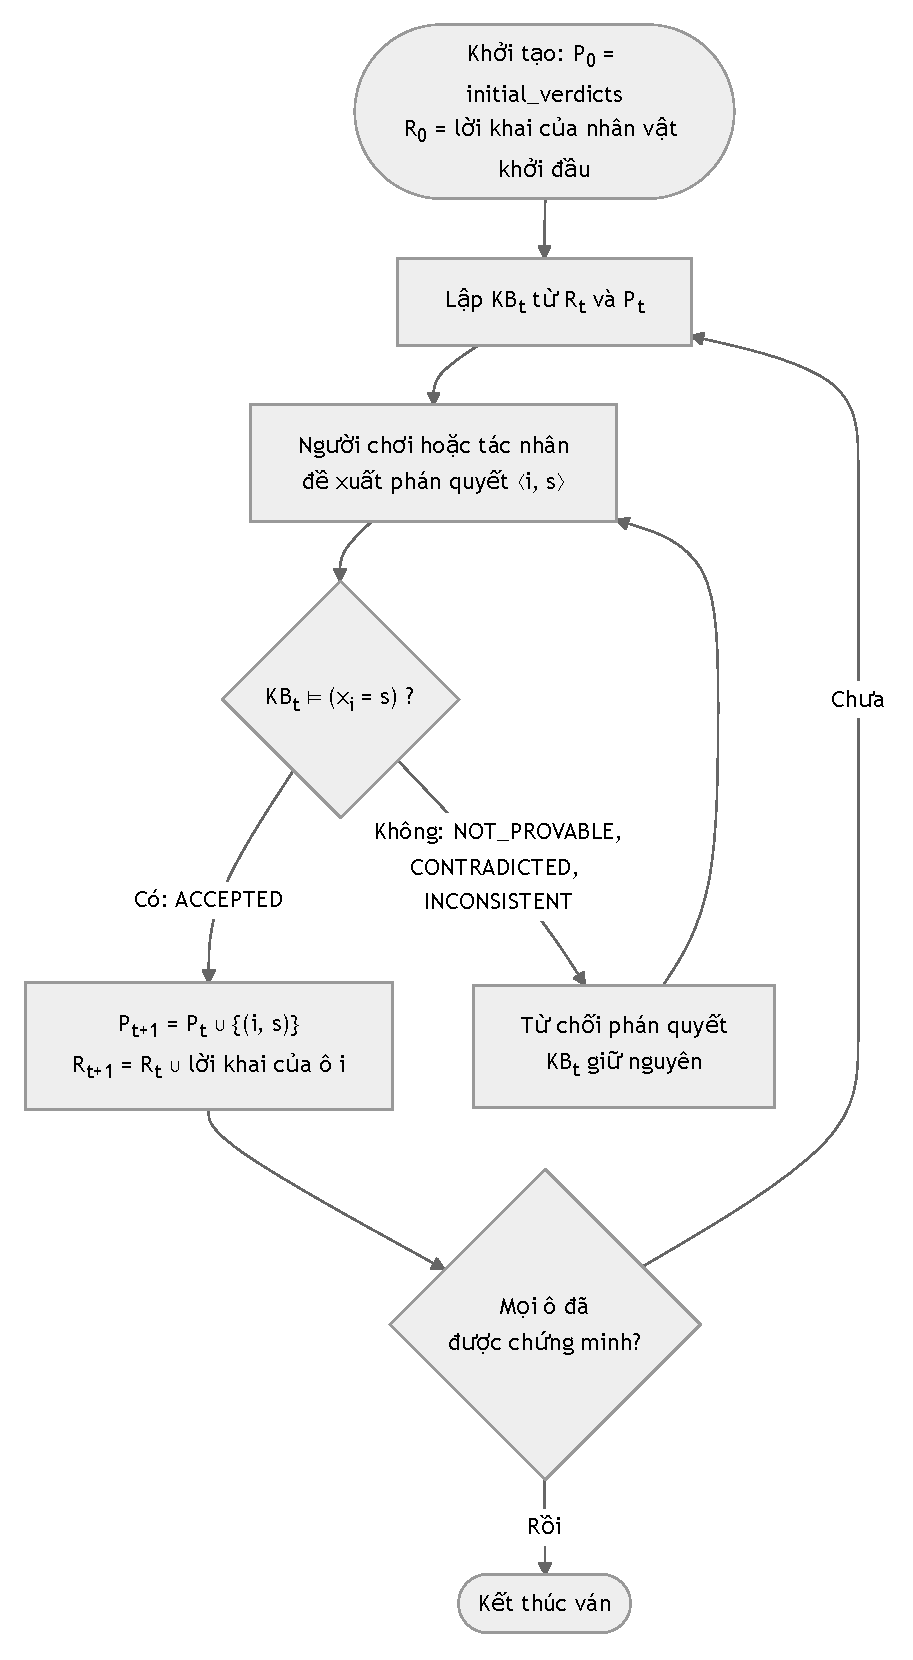
\includegraphics[width=0.62\linewidth]{figures/reveal_loop.pdf}
  \caption{Vòng lặp phán quyết và lật mở lời khai. Chỉ phán quyết được
    $\mathit{KB}_t$ suy ra tất yếu mới làm thay đổi trạng thái; mọi phán quyết
    khác bị từ chối và $\mathit{KB}_t$ giữ nguyên.}
  \label{fig:reveal_loop}
\end{figure}

\subsection{Điều kiện chấp nhận kết luận và luật không đoán}
\label{sec:verdict_acceptance}

Mục này nêu tiêu chí hình thức để Game Engine chấp nhận một phán quyết, cách
quy tiêu chí đó về bài toán SAT, và luật ``không đoán'' mà tiêu chí này bảo
đảm.

\paragraph{Điều kiện suy diễn.}
Phán quyết $\langle i, s\rangle$ được chấp nhận tại thời điểm $t$ khi và chỉ
khi nó là hệ quả logic của tri thức công khai:
\begin{equation}
  \mathit{KB}_t \models (x_i = s)
  \iff
  \mathit{KB}_t \land (x_i \ne s) \text{ không thỏa được}.
  \label{eq:entailment}
\end{equation}
Vế phải của \eqref{eq:entailment} là một truy vấn SAT. Hàm
\texttt{has\_solution(state, assumption)} của bộ kiểm tra trả về
\texttt{True} khi $\mathit{KB}_t$ cùng giả thiết tùy chọn thỏa được. Game
Engine gọi hàm này hai lần,
\begin{equation}
  a = \mathrm{SAT}\bigl(\mathit{KB}_t \land (x_i = s)\bigr),
  \qquad
  b = \mathrm{SAT}\bigl(\mathit{KB}_t \land (x_i \ne s)\bigr),
\end{equation}
và phân loại kết quả theo cặp $(a, b)$. Truy vấn $a$ là cần thiết dù
\eqref{eq:entailment} chỉ dùng $b$: nó tách trường hợp phán quyết bị bác bỏ
khỏi trường hợp chính $\mathit{KB}_t$ mâu thuẫn.

\paragraph{Phân loại kết quả.}
Hình~\ref{fig:verdict_outcome} mô tả thứ tự kiểm tra trong
\texttt{submit\_verdict}, và Bảng~\ref{tab:submit_outcome} liệt kê sáu kết quả
có thể. Chỉ kết quả \texttt{ACCEPTED} làm thay đổi trạng thái ván chơi; năm kết
quả còn lại trả về ảnh chụp công khai không đổi.

\begin{figure}[htbp]
  \centering
  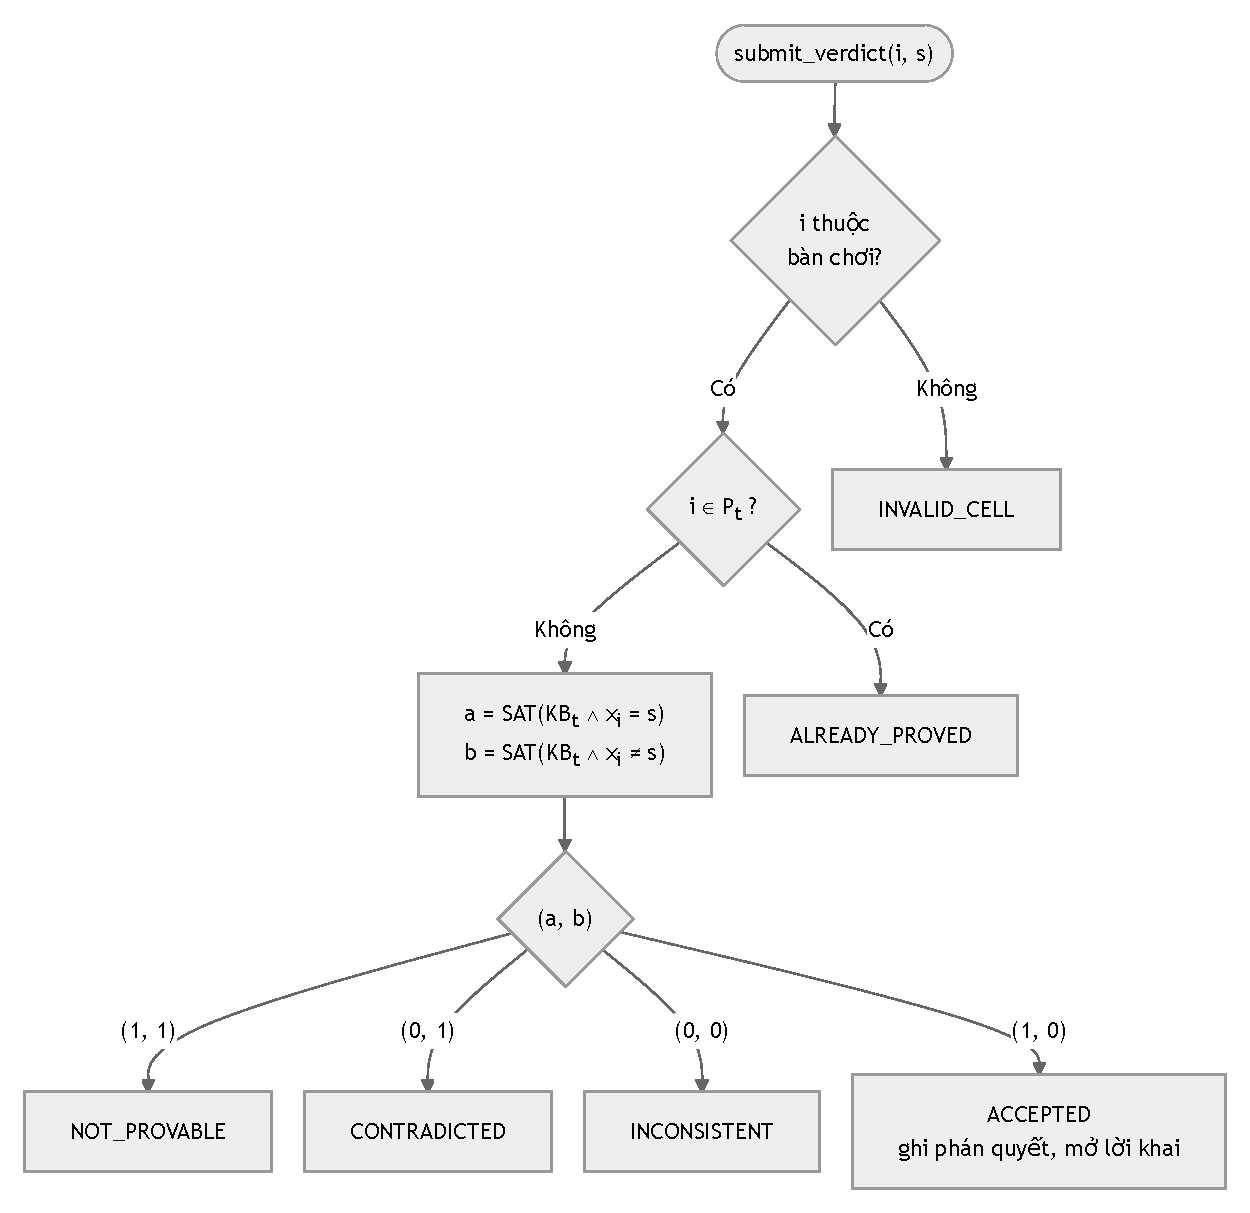
\includegraphics[width=0.78\linewidth]{figures/verdict_outcome.pdf}
  \caption{Thứ tự kiểm tra khi nộp phán quyết $\langle i, s\rangle$. Hai kiểm
    tra đầu không cần bộ giải; bốn kết quả cuối được quyết định bởi hai truy vấn
    SAT $a$ và $b$.}
  \label{fig:verdict_outcome}
\end{figure}

\begin{table}[htbp]
  \centering
  \caption{Các kết quả của \texttt{submit\_verdict}}
  \label{tab:submit_outcome}
  \begin{tabularx}{\textwidth}{ll>{\raggedright\arraybackslash}X}
    \toprule
    \textbf{Kết quả} & \textbf{Điều kiện} & \textbf{Ý nghĩa} \\
    \midrule
    \texttt{INVALID\_CELL}   & $i \notin \mathcal{C}$          & Ô không thuộc bàn chơi \\
    \texttt{ALREADY\_PROVED} & $i$ đã có trong $\mathcal{P}_t$ & Ô đã được chứng minh trước đó \\
    \texttt{ACCEPTED}        & $a \land \neg b$                & $\mathit{KB}_t \models (x_i = s)$; ghi phán quyết và lật lời khai của ô $i$ \\
    \texttt{NOT\_PROVABLE}   & $a \land b$                     & Cả hai trạng thái còn khả dĩ; chưa đủ bằng chứng \\
    \texttt{CONTRADICTED}    & $\neg a \land b$                & $\mathit{KB}_t \models (x_i \ne s)$; phán quyết sai \\
    \texttt{INCONSISTENT}    & $\neg a \land \neg b$           & $\mathit{KB}_t$ không thỏa được; bản đồ bị lỗi \\
    \bottomrule
  \end{tabularx}
\end{table}

\paragraph{Luật không đoán.}
Kết quả \texttt{NOT\_PROVABLE} hiện thực luật trung tâm của Griductive: một phán
quyết đúng với lời giải nhưng chưa được $\mathit{KB}_t$ suy ra vẫn bị từ chối.
Trò chơi gốc mô tả luật này là ``bạn không bao giờ phải đoán: tại mọi thời
điểm, luôn có ít nhất một phán quyết suy ra được từ các lời khai''
\cite{griductive_rules}. Luật có hai mặt. Về phía người chơi, mỗi phán quyết
được chấp nhận đều kèm một chứng minh, nên trò chơi là bài toán suy diễn chứ
không phải thử và sai. Về phía người thiết kế, mỗi bản đồ phải bảo đảm rằng tại
mọi trạng thái chưa hoàn thành luôn tồn tại ít nhất một ô thỏa
\eqref{eq:entailment}. Hàm \texttt{validate\_puzzle} kiểm chứng điều kiện thứ
hai bằng cách cho một người chơi hoàn hảo đi qua Game Engine thật và báo lỗi
nếu có một lượt không phán quyết nào được chấp nhận.


\section{Thiết kế và triển khai Game Engine}
% Note: Người phụ trách Game Engine trình bày cấu trúc và luồng thực thi.

% Tiêu đề \paragraph nằm trên một dòng riêng, nội dung bắt đầu ở dòng dưới.
% Đặt trong nhóm để chỉ áp dụng cho phần này.
\begingroup
\titleformat{\paragraph}[hang]{\normalfont\bfseries}{}{0pt}{}
\titlespacing*{\paragraph}{0pt}{8pt}{2pt}

\subsection{Kiến trúc tổng thể}
% Note: Vẽ sơ đồ UI, API, Engine, Agent và SAT Solver; mô tả trách nhiệm và dữ liệu trao đổi.


\subsection{Game Object và cấu trúc dữ liệu bàn chơi}
\label{sec:game_objects}
\begin{sloppypar}

Module \texttt{GameObject/objects.py} khai báo năm lớp mô tả một đề bài. Tất cả
đều là \texttt{dataclass(frozen=True)}: không đối tượng nào sửa được sau khi
tạo, và các tập hợp bên trong được lưu bằng \texttt{tuple} thay vì
\texttt{list}. Nhờ đó một \texttt{PuzzleDefinition} được dùng chung an toàn
giữa nhiều ván, giữa engine và bộ kiểm tra, mà không cần sao chép. Toàn bộ
trạng thái thay đổi được của ván tách riêng sang \texttt{GameState}
(Mục~\ref{sec:game_state}).

\begin{table}[htbp]
  \centering\small
  \caption{Các lớp dữ liệu trong \texttt{objects.py}}
  \label{tab:game_objects}
  \begin{tabularx}{\textwidth}{l>{\raggedright\arraybackslash}X}
    \toprule
    \textbf{Lớp} & \textbf{Trường và ý nghĩa} \\
    \midrule
    \texttt{Cell} & \texttt{id: int}; \texttt{coordinates: (int, int)} là
      (hàng, cột) đánh số từ $0$; \texttt{character\_name}; \texttt{profession} \\
    \texttt{Board} & \texttt{cells}: bộ hai chiều các \texttt{Cell}, theo hàng.
      Thuộc tính tính toán \texttt{height}, \texttt{width}, \texttt{cell\_count} \\
    \texttt{Verdict} & \texttt{cell\_id}; \texttt{is\_criminal: bool}
      (\texttt{True} là tội phạm) \\
    \texttt{Clue} & \texttt{id}; \texttt{source\_cell\_id: int | None}
      (\texttt{None} là lời khai công khai từ đầu); \texttt{constraint};
      \texttt{description\_nl} là câu tiếng Việt hiển thị cho người chơi \\
    \texttt{PuzzleDefinition} & \texttt{id} (ví dụ \texttt{medium-4x4-harbor});
      \texttt{board}; \texttt{clues}; \texttt{solution} là đáp án đầy đủ;
      \texttt{initial\_verdicts} là các phán quyết có sẵn khi bắt đầu \\
    \bottomrule
  \end{tabularx}
\end{table}

\paragraph{Định danh và tọa độ.}
Mỗi ô có hai cách định vị: định danh phẳng \texttt{id} (khóa dùng chung giữa
engine, bộ kiểm tra và API) và \texttt{coordinates} (dùng khi cần quan hệ hình
học). \texttt{Board} chỉ lưu lưới ô và suy ra kích thước từ đó:
\texttt{height} là số hàng, \texttt{width} là độ dài hàng đầu, và
\texttt{cell\_count} $= \texttt{width}\times\texttt{height}$. Lớp này không tự
kiểm tra lưới có hình chữ nhật hay tọa độ khai báo có khớp vị trí. Hai điều kiện
đó được \texttt{validate\_puzzle} kiểm tra trong hàm \texttt{\_check\_grid}. Kiểm
tra này cần thiết vì \texttt{BruteForceChecker} và \texttt{CNFEncoder} tìm láng
giềng cạnh của \texttt{ConnectedConstraint} dựa trên \texttt{coordinates}, chứ
không dựa trên vị trí trong mảng.

\paragraph{Dựng bàn chơi cho các bản đồ.}
Sáu bản đồ dùng chung hàm \texttt{make\_board(size)} trong
\texttt{Maps/common.py}. Hàm lấy $\texttt{size}^2$ nhân vật đầu tiên từ danh
sách cố định $25$ cặp (tên, nghề), gán \texttt{id} tăng dần từ $0$ và tọa độ
\texttt{divmod(id, size)}, rồi cắt thành từng hàng. Vì vậy định danh luôn theo
thứ tự hàng và $\texttt{id} = r \cdot W + c$, đúng với công thức
\eqref{eq:cell_id}. Mỗi module bản đồ khai báo thêm tập \texttt{CRIMINALS},
các \texttt{Clue}, và dựng \texttt{solution} bằng
\texttt{Verdict(i, i in CRIMINALS)} cho mọi ô.

\paragraph{Truy vấn trên bàn chơi.}
Module \texttt{board\_utils.py} cung cấp bốn hàm trả về bộ định danh ô:
\texttt{row\_ids(board, r)}, \texttt{column\_ids(board, c)},
\texttt{profession\_ids(board, p)}, và \texttt{neighbor\_ids(board, i)} trả về
tối đa tám ô lân cận kể cả đường chéo, không gồm chính ô $i$. Hàm cuối duyệt
lưới tìm ô $i$, rồi cắt lát các hàng và cột trong khoảng
$[\max(0, r-1),\, r+2)$ và $[\max(0, c-1),\, c+2)$, nên tự xử lý ô ở biên và
góc. Ô không tồn tại gây \texttt{ValueError}. Các hàm này mô tả đúng những tập
đích mà lời khai trong bản đồ dùng tới (hàng, cột, lân cận). Tuy nhiên, ở phiên
bản hiện tại các module bản đồ ghi tường minh tập định danh trong từng ràng buộc,
ví dụ \texttt{Count((3, 4, 5))} cho hàng 2 của lưới $3\times3$, và không module
nào gọi tới \texttt{board\_utils}.
\end{sloppypar}

\subsection{Biểu diễn Clue và Constraint}
% Note: Mô tả cấu trúc Clue, source_cell_id và các kiểu Constraint; tập trung cách cài đặt, tránh lặp lại ngữ nghĩa ở phần mô hình.


\subsection{Game State và Public State}
% Note: Giải thích trạng thái nội bộ, verdict đã xác nhận, clue đã mở và dữ liệu được phép công khai.


\subsection{Luồng xử lý verdict, reveal và restart}
\label{sec:engine_flow}
\begin{sloppypar}

\texttt{GameEngine} cung cấp ba thao tác công khai là \texttt{get\_public\_state},
\texttt{submit\_verdict} và \texttt{restart}. Mục này mô tả luồng thực thi của
các thao tác đó, còn điều kiện logic tương ứng với từng kết quả đã được hình
thức hóa ở Mục~\ref{sec:verdict_acceptance} (Bảng~\ref{tab:submit_outcome}).

\paragraph{Khởi tạo}
Hàm khởi tạo nhận vào một \texttt{PuzzleDefinition} cùng một bộ kiểm tra, tính
trước tập định danh ô hợp lệ dưới dạng \texttt{frozenset} để việc kiểm tra một ô
có tồn tại hay không chỉ tốn $O(1)$, rồi gọi \texttt{\_initial\_state()}. Hàm
này tạo một \texttt{GameState} rỗng và áp dụng lần lượt các phán quyết trong
\texttt{initial\_verdicts} thông qua chính hàm \texttt{\_apply\_proof} vốn dùng
cho phán quyết thông thường. Nhờ vậy, nhân vật khởi đầu vừa được đánh dấu là đã
chứng minh, vừa có lời khai được lật sẵn, mà không cần viết thêm mã xử lý riêng
cho trạng thái ban đầu. Lưu ý rằng engine không gọi bộ kiểm tra đối với các
phán quyết ban đầu, vì tính đúng đắn của chúng đã được \texttt{validate\_puzzle}
xác nhận từ trước khi đối chiếu với đáp án.

\paragraph{Nộp phán quyết}
Luồng xử lý của \texttt{submit\_verdict(cell\_id, status)} được trình bày trong
Thuật toán~\ref{alg:submit_verdict}. Hai bước kiểm tra đầu tiên không cần đến
bộ giải nên được thực hiện trước; sau đó engine gọi \texttt{has\_solution} đúng
hai lần trên \emph{cùng một} ảnh chụp công khai, một lần với giả thiết của người
chơi và một lần với giả thiết ngược lại. Kết quả trong mọi trường hợp đều được
đóng gói thành \texttt{SubmitResult(verdict, outcome, public\_state)}, và engine
không ném ngoại lệ cho nước đi sai. Việc ánh xạ kết quả sang mã HTTP được giao cho
API, trong đó hiện chỉ có \texttt{INVALID\_CELL} được chuyển thành HTTP~404, còn
năm kết quả còn lại được trả về với HTTP~200 kèm trường \texttt{outcome}.

\begin{algorithm}[htbp]
  \caption{\texttt{GameEngine.submit\_verdict}}
  \label{alg:submit_verdict}
  \begin{algorithmic}[1]
    \Require ô $i$, trạng thái $s$
    \Ensure \texttt{SubmitResult}
    \State $P \gets \Call{GetPublicState}{}$ \Comment{ảnh chụp trước nước đi}
    \If{$i \notin$ tập ô hợp lệ} \Return $(\langle i,s\rangle, \texttt{INVALID\_CELL}, P)$ \EndIf
    \If{$i \in \texttt{proved\_statuses}$} \Return $(\langle i,s\rangle, \texttt{ALREADY\_PROVED}, P)$ \EndIf
    \State $a \gets \textsc{HasSolution}(P, \langle i, s\rangle)$
    \State $b \gets \textsc{HasSolution}(P, \langle i, \neg s\rangle)$
    \If{$a \land b$} \Return $(\cdot, \texttt{NOT\_PROVABLE}, P)$ \EndIf
    \If{$\neg a \land b$} \Return $(\cdot, \texttt{CONTRADICTED}, P)$ \EndIf
    \If{$\neg a \land \neg b$} \Return $(\cdot, \texttt{INCONSISTENT}, P)$ \EndIf
    \State $\Call{ApplyProof}{\mathit{state}, i, s}$ \Comment{chỉ nhánh $a \land \neg b$ tới đây}
    \State \Return $(\langle i,s\rangle, \texttt{ACCEPTED}, \Call{GetPublicState}{})$
  \end{algorithmic}
\end{algorithm}

Từ thuật toán có thể thấy chỉ kết quả \texttt{ACCEPTED} mới ghi vào trạng thái
ván. Năm kết quả còn lại đều trả về chính ảnh chụp $P$ được dựng ở dòng~1, nên
một nước đi sai không để lại bất kỳ dấu vết nào trong \texttt{GameState}; các ca
kiểm thử \texttt{test\_submit\_*} khẳng định điều này bằng cách so sánh
\texttt{engine.get\_public\_state()} với ảnh chụp trước nước đi. Bên cạnh đó,
\texttt{submit\_verdict} hoàn toàn không đọc \texttt{PuzzleDefinition.solution},
vì vậy một phán quyết dù đúng với đáp án nhưng chưa suy ra được từ thông tin
công khai vẫn nhận kết quả \texttt{NOT\_PROVABLE}. Engine cũng không dùng bộ nhớ
đệm: mỗi lần nộp tốn đúng hai lời gọi \texttt{has\_solution}, và bộ kiểm tra dựng
lại toàn bộ ràng buộc từ ảnh chụp ở mỗi lần gọi. Cách làm này đơn giản và luôn
nhất quán với trạng thái hiện tại, còn chi phí của nó được đo ở Mục~7.

\paragraph{Lật lời khai}
Khi một phán quyết được chấp nhận, hàm \texttt{\_apply\_proof(state, i, s)} hiện
thực quy tắc \eqref{eq:reveal} qua hai bước: ghi \texttt{state.proved\_statuses[i]
= s}, sau đó thêm vào \texttt{state.revealed\_clue\_ids} định danh của mọi lời
khai có \texttt{source\_cell\_id} bằng $i$. Bước lật không phụ thuộc vào giá trị
$s$, do đó lời khai của tội phạm cũng được lật như lời khai của người vô tội. Vì
ảnh chụp trả về sau \texttt{ACCEPTED} đã chứa lời khai mới, lời gọi kế tiếp, dù
đến từ người chơi hay tác nhân, đều có thể sử dụng ngay thông tin này. Ca kiểm
thử \texttt{test\_revealed\_clue\_makes\_new\_cell\_provable} kiểm tra đúng chuỗi
sự kiện đó, khi một ô ban đầu nhận \texttt{NOT\_PROVABLE} trở thành
\texttt{ACCEPTED} sau khi lời khai mới được lật.

\paragraph{Hoàn tất ván}
Engine không có trạng thái ``kết thúc'' riêng; ván được xem là hoàn tất khi
\texttt{PublicState.is\_complete} đúng, tức là mọi ô đều đã có mặt trong
\texttt{proved\_statuses}. Kể từ thời điểm đó, mọi lần nộp tiếp theo đều nhận
\texttt{ALREADY\_PROVED} nên trạng thái ván không thể thay đổi thêm. API trả về
trường \texttt{is\_complete} trong mỗi phản hồi để giao diện hiển thị màn hình
kết thúc, còn \texttt{DeductiveAgent.next\_move} trả về \texttt{SOLVED} khi không
còn ô nào chưa được chứng minh.

\paragraph{Khởi động lại}
Hàm \texttt{restart()} thay \texttt{self.\_state} bằng một kết quả mới của
\texttt{\_initial\_state()} và trả về ảnh chụp tương ứng. Do trạng thái được dựng
lại từ \texttt{PuzzleDefinition} bất biến, ván chơi luôn trở về đúng
$(\mathcal{R}_0, \mathcal{P}_0)$ bất kể trước đó đã đi bao nhiêu nước, trong khi
các ảnh chụp cũ đã phát ra vẫn không bị ảnh hưởng vì mỗi ảnh chụp giữ bản sao
riêng. Ở phía API, thao tác nạp bản đồ khác (\nolinkurl{/api/game/load}) không
gọi \texttt{restart} mà tạo hẳn một \texttt{GameEngine} mới rồi thay vào
\texttt{app.state.engine}.
\end{sloppypar}

\subsection{Kiểm soát thông tin công khai và thông tin ẩn}
% Note: Trình bày cách ngăn đáp án và clue chưa mở xuất hiện trong Public State, phản hồi API hoặc đầu vào của Agent.


\endgroup

\section{Game Agent: CNF Encoding và thuật toán suy luận}
% Note: Nhóm Game Agent viết CNF Encoder, DPLL và Deductive Logic Agent; chỉ chia đến subsection.

\subsection{Luồng xử lý từ Public State đến verdict}
\label{sec:agent_pipeline}
\begin{sloppypar}

Tác nhân suy luận của dự án được tách thành ba tầng độc lập.
\texttt{DeductiveAgent} quyết định \emph{hỏi gì} và \emph{nộp gì};
\texttt{DPLLChecker} dựng cơ sở tri thức và trả lời câu hỏi thỏa được hay
không; \texttt{CNFEncoder} cùng hàm \texttt{solve} của bộ giải DPLL đảm nhận
phần tính toán logic. Ba tầng chỉ giao tiếp qua giao diện
\texttt{ConstraintChecker}, gồm đúng một phương thức
\begin{center}
  \texttt{has\_solution(public\_state, assumption=None) -> bool},
\end{center}
trả về \texttt{True} khi $\mathit{KB}_t$ (cùng giả thiết tạm thời nếu có) thỏa
được. Tác nhân nhận bộ kiểm tra qua hàm khởi tạo, nên cùng một mã tác nhân có
thể chạy trên \texttt{DPLLChecker} khi chơi thật hoặc trên
\texttt{BruteForceChecker} khi đối chứng trong kiểm thử. Các mục sau dùng biến
$x_i$ như ở Mục~\ref{sec:prop_vars}; literal $x_i$ ứng với ký hiệu $C_i$ (ô $i$
là tội phạm) của đề bài và của Mục~4.2.

\paragraph{Năm bước của một lượt suy luận.}
Mỗi lượt bắt đầu từ một ảnh chụp \texttt{PublicState} và kết thúc bằng một
phán quyết được Game Engine chấp nhận, hoặc bằng kết luận rằng không còn phán
quyết nào chứng minh được. Bảng~\ref{tab:agent_pipeline} nêu đầu vào và đầu
ra của từng bước.

\begin{enumerate}
  \item \textbf{Lấy thông tin công khai.} Tác nhân gọi
    \texttt{GameEngine.get\_public\_state()} và nhận ảnh chụp chỉ đọc gồm bàn
    chơi, tập lời khai đã lật $\mathcal{R}_t$ và tập phán quyết đã chứng minh
    $\mathcal{P}_t$. Ảnh chụp không chứa $\sigma^\star$ hay lời khai chưa lật
    (Mục~\ref{sec:knowledge_base}), nên mọi bước phía sau chỉ có thể dùng
    thông tin công khai.
  \item \textbf{Xác định ô cần xét.} Tác nhân duyệt bàn chơi theo thứ tự hàng
    và lấy tập ô chưa chứng minh
    $U_t = \mathcal{C} \setminus \{\, i : \langle i, s\rangle \in \mathcal{P}_t \,\}$,
    giữ thứ tự định danh tăng dần. Thứ tự cố định làm cho toàn bộ quá trình
    suy luận tất định: chạy lại cùng một bản đồ luôn cho cùng một trace.
  \item \textbf{Dựng $\mathit{KB}_t$ dưới dạng CNF.} Mỗi lần
    \texttt{has\_solution} được gọi, \texttt{DPLLChecker} tạo một
    \texttt{CNFEncoder} mới trên bàn chơi, mã hóa lần lượt ràng buộc của mọi lời
    khai trong $\mathcal{R}_t$, thêm một mệnh đề đơn vị cho mỗi phán quyết trong
    $\mathcal{P}_t$ theo \eqref{eq:kb}, rồi thêm mệnh đề đơn vị của giả thiết
    $x_i = s$ nếu có. Số biến truyền cho bộ giải là
    \texttt{next\_variable}$-1$, gồm $|\mathcal{C}|$ biến ô và các biến phụ
    trợ vừa được cấp phát. Vì công thức được dựng lại từ đầu, giả thiết của
    truy vấn trước không bao giờ rò sang truy vấn sau.
  \item \textbf{Truy vấn SAT.} Hàm \texttt{solve(cnf, n)} trả về một phép gán
    thỏa mãn hoặc \texttt{None} (Mục~4.3); \texttt{DPLLChecker} rút gọn kết quả
    thành một giá trị Boolean. Với mỗi ô $i \in U_t$, tác nhân hỏi hai câu
    $\mathrm{SAT}(\mathit{KB}_t \land x_i)$ và
    $\mathrm{SAT}(\mathit{KB}_t \land \neg x_i)$, và ghi mỗi câu hỏi vào một
    bản ghi \texttt{Query(assumption, satisfiable)}.
  \item \textbf{Phân loại và chọn verdict.} Cặp câu trả lời được phân loại
    thành \texttt{CRIMINAL}, \texttt{INNOCENT} hoặc \texttt{UNKNOWN} theo
    Mục~\ref{sec:entailment_classification}. Ô đầu tiên (theo thứ tự định danh)
    có nhãn khác \texttt{UNKNOWN} cho ra phán quyết $\langle i, s\rangle$, được
    gửi tới \texttt{GameEngine.submit\_verdict}. Engine tự kiểm tra lại bằng hai
    truy vấn của chính nó, lật lời khai của ô $i$ và trả về ảnh chụp mới
    (Mục~\ref{sec:deductive_agent}).
\end{enumerate}

\begin{table}[htbp]
  \centering\small
  \caption{Đầu vào và đầu ra của từng bước trong một lượt suy luận}
  \label{tab:agent_pipeline}
  \begin{tabularx}{\textwidth}{c>{\raggedright\arraybackslash}p{3.5cm}%
      >{\raggedright\arraybackslash}X>{\raggedright\arraybackslash}X}
    \toprule
    \textbf{Bước} & \textbf{Thành phần} & \textbf{Đầu vào} & \textbf{Đầu ra} \\
    \midrule
    1 & \texttt{GameEngine} & Trạng thái nội bộ \texttt{GameState}
      & \texttt{PublicState} chỉ đọc: bàn chơi, $\mathcal{R}_t$, $\mathcal{P}_t$ \\
    2 & \texttt{DeductiveAgent} & \texttt{PublicState}
      & Danh sách ô chưa chứng minh $U_t$, theo thứ tự định danh \\
    3 & \texttt{DPLLChecker}, \texttt{CNFEncoder}
      & \texttt{PublicState}, giả thiết \texttt{Verdict} hoặc \texttt{None}
      & CNF dạng DIMACS của $\mathit{KB}_t \land (x_i = s)$ và số biến $n$ \\
    4 & \texttt{solve} (DPLL) & CNF, $n$
      & Phép gán thỏa mãn hoặc \texttt{None}, rút gọn thành \texttt{bool} \\
    5 & \texttt{DeductiveAgent} & Hai giá trị \texttt{bool} cho mỗi ô
      & Nhãn của ô; \texttt{Move} gồm trạng thái, phán quyết và danh sách
        \texttt{Query} \\
    \bottomrule
  \end{tabularx}
\end{table}

\paragraph{Ba điểm vào của tác nhân.}
Cùng một đường ống trên được dùng qua ba phương thức.
\texttt{next\_move(state)} chạy năm bước cho tới khi tìm được ô đầu tiên chứng
minh được, rồi dừng ngay. API dùng phương thức này cho chức năng gợi ý
(\texttt{GET /api/game/hint}), nên gợi ý không làm thay đổi ván chơi.
\texttt{classify\_all(state)} cũng chạy các bước đó nhưng không dừng sớm, và
trả về nhãn của \emph{mọi} ô chưa chứng minh; nó cho thấy toàn bộ những gì
$\mathit{KB}_t$ suy ra được tại một thời điểm. Cuối cùng,
\texttt{solve(engine)} lặp \texttt{next\_move} và nộp phán quyết cho tới khi
ván kết thúc. API dùng phương thức này cho chức năng tự giải
(\texttt{POST /api/game/auto-solve}).

\paragraph{Tác nhân không được tin tưởng mặc định.}
Đường ống có hai lớp kiểm tra độc lập. Tác nhân chỉ nộp phán quyết mà nó đã tự
chứng minh, nhưng Game Engine không dựa vào điều đó: \texttt{submit\_verdict}
chạy lại hai truy vấn trên cùng $\mathit{KB}_t$ và chỉ ghi nhận khi kết quả là
\texttt{ACCEPTED} (Bảng~\ref{tab:submit_outcome}). Cách bố trí này tốn thêm hai
lời gọi bộ giải cho mỗi phán quyết. Trên bản đồ Khu chợ chẳng hạn, tác nhân gọi
bộ giải $29$ lần và Game Engine gọi thêm $16$ lần, tổng cộng $45$ lần
(Bảng~\ref{tab:benchmark_raw}). Đổi lại, một lỗi trong tác nhân không thể đưa
ván chơi vào trạng thái sai: phán quyết không chứng minh được sẽ bị từ chối như
khi người chơi nộp.
\end{sloppypar}

\subsection{CNF Encoder}
% Note: Trình bày ánh xạ biến/literal/clause; dẫn xuất từng bước ít nhất một binary clue và một counting clue, cách mã hóa clue còn lại, số biến phụ và clause.


\subsection{DPLL SAT Solver}
% Note: Mô tả SAT/UNSAT, unit propagation, đơn giản hóa CNF, chọn biến, phân nhánh, quay lui; bổ sung giả mã và độ phức tạp đúng với cài đặt.
Sau khi các ràng buộc của các ván chơi đã được ãm hóa sang dạng chuẩn hội CNF, nhóm sử dụng thuật toán Davis--Putnam--Logemann--Loveland (DPLL) để kiểm tra công thức có nghiệm hay không. 
Trong cài đặt, mỗi literal được biểu diễn bằng một số nguyên có dấu. Chẳng hạn, \texttt{3} biểu diễn $x_3$ và \text{-3} biểu diễn $\neg x_3$. Mỗi mệnh đề là
một bộ các literal, còn công thức CNF là một bộ các mệnh đề. Hàm \texttt{solve} nhận công thức CNF và số biến, sau đó trả về một phép gán đầy đủ nếu công thức thỏa hoặc \texttt{None} nếu công thức vô nghiệm.

Ở mỗi nút tìm kiếm, bộ giải được thực hiện lan truyền đơn vị trước khi phân nhánh.
Nếu một mệnh đề chỉ còn literal $\ell$, mọi nghiệm của công thức tại nút đó đều phải làm cho $\ell$ đúng. 
Bộ giải ghi nhận phép gán này, bỏ các mệnh đề chứa $\ell$
vì chúng đã được thỏa, rồi xóa $\neg\ell$ khỏi các mệnh đề còn lại.
Quá trình được lặp lại vì một lần đơn giản hóa có thể tạo ra mệnh đề
đơn vị mới. Nếu xuất hiện một mệnh đề rỗng, nhánh hiện tại vô nghiệm.
Nếu công thức không còn mệnh đề nào, phép gán hiện tại đã thỏa toàn bộ
các ràng buộc.
Khi lan truyền đơn vị dừng mà công thức vẫn còn mệnh đề, cài đặt của
nhóm chọn biến có chỉ số nhỏ nhất còn xuất hiện trong công thức.
Bộ giải lần lượt thử giá trị \texttt{True} và \texttt{False}. Mỗi
nhánh sử dụng một bản sao của phép gán hiện tại, nhờ đó các giá trị
phát sinh ở nhánh thất bại không ảnh hưởng đến nhánh tiếp theo.
Thuật toán~\ref{alg:dpll-search} mô tả hàm tìm kiếm đệ quy.

\begin{algorithm}[htbp]
    \caption{Tìm kiếm nghiệm bằng DPLL}
    \label{alg:dpll-search}
    \begin{algorithmic}[1]
        \Require Công thức CNF $F$, phép gán hiện tại $A$
        \Ensure Một phép gán thỏa mãn hoặc $\bot$ nếu vô nghiệm
        \State $R \gets$ \Call{LanTruyenDonVi}{$F,A$}
        \If{$R=\bot$}
            \State \Return $\bot$
        \EndIf
        \State $(F,A) \gets R$
        \If{$F$ không còn mệnh đề}
            \State \Return $A$
        \EndIf
        \State $x \gets$ biến có chỉ số nhỏ nhất còn xuất hiện trong $F$
        \For{$b$ lần lượt nhận giá trị $\mathrm{True},\mathrm{False}$}
            \State $A' \gets$ bản sao của $A$ có bổ sung phép gán $x=b$
            \State $F' \gets$ công thức thu được khi đơn giản hóa $F$ theo $x=b$
            \State $R \gets$ \Call{DPLL}{$F',A'$}
            \If{$R\neq\bot$}
                \State \Return $R$
            \EndIf
        \EndFor
        \State \Return $\bot$
    \end{algorithmic}
\end{algorithm}

Xét công thức
\[
F=(\neg x_1 \lor x_2)
  \land(\neg x_1 \lor \neg x_2)
  \land(x_1 \lor x_3).
\]
Ban đầu, $F$ chưa có mệnh đề đơn vị nên bộ giải chọn $x_1$. Khi thử
$x_1=\mathrm{True}$, hai mệnh đề đầu lần lượt rút gọn thành $x_2$ và
$\neg x_2$. Hai yêu cầu này mâu thuẫn, do đó bộ giải quay lui và thử
$x_1=\mathrm{False}$. Lúc này, hai mệnh đề đầu đã được thỏa, còn mệnh
đề cuối rút gọn thành $x_3$. Lan truyền đơn vị gán
$x_3=\mathrm{True}$ và công thức không còn mệnh đề nào. Vì $x_2$
chưa cần được gán, hàm \texttt{solve} điền giá trị \texttt{False}
để trả về phép gán đầy đủ
$(x_1,x_2,x_3)=(\mathrm{False},\mathrm{False},\mathrm{True})$.

Lan truyền đơn vị bảo toàn các nghiệm vì mỗi giá trị được gán ở
bước này đều do một mệnh đề bắt buộc. Khi phải phân nhánh, hai giá trị
của biến được chọn bao phủ mọi khả năng của biến đó. Vì vậy, nếu cả
hai nhánh đều thất bại thì công thức tại nút hiện tại vô nghiệm.
Với $n$ biến, kể cả biến phụ do bộ mã hóa sinh ra, cây tìm kiếm có
thể có $O(2^n)$ nút trong trường hợp xấu nhất. Tại mỗi nút, cài đặt
còn phải quét các mệnh đề và tạo công thức rút gọn cho từng phép gán.
Lan truyền đơn vị giúp giảm số lần phân nhánh bằng cách xác định trước
những giá trị đã bị ràng buộc ép buộc.

Trong Griductive Solver, lớp \texttt{DPLLChecker} xây dựng cơ sở tri
thức $KB$ từ các manh mối đã mở và các nhận định đã được chứng minh.
Để xét một ô, hệ thống lần lượt kiểm tra $KB\land x$ và
$KB\land\neg x$, trong đó $x$ biểu diễn việc ô đó có tội. Chẳng hạn,
nếu $KB\land x$ vô nghiệm và $KB\land\neg x$ thỏa được, mọi nghiệm
phù hợp với thông tin công khai đều xác định ô đó vô tội. Kết quả
này là căn cứ để agent đưa ra gợi ý hoặc để engine chấp nhận nhận
định của người chơi.
\subsection{Entailment classification}
% Note: Lập bảng SAT(KB AND x) và SAT(KB AND NOT x) để phân loại Criminal, Innocent, Unknown và KB không nhất quán; giải thích phép suy ra bằng phản chứng.


\subsection{Uniqueness checking}
\label{sec:uniqueness_checking}
\begin{sloppypar}
% Tiêu đề \paragraph nằm trên một dòng riêng; sloppypar là một nhóm nên cấu
% hình này chỉ áp dụng trong mục này.
\titleformat{\paragraph}[hang]{\normalfont\bfseries}{}{0pt}{}
\titlespacing*{\paragraph}{0pt}{8pt}{2pt}

Một bản đồ Griductive hợp lệ phải có đúng một lời giải, bởi nếu tồn tại hai cấu
hình tội trạng cùng thỏa mọi lời khai thì không có cách nào phân biệt chúng bằng
suy luận, và người chơi buộc phải đoán. Trong hệ thống, tính duy nhất của nghiệm
được kiểm tra bởi hàm \texttt{\_check\_unique\_solution} trong
\texttt{BackEnd/GameEngine/validation.py}. Hàm này là bước thứ hai của
\texttt{validate\_puzzle}, chạy sau bước kiểm tra cấu trúc (và kiểm tra mỗi ô có
đúng một lời khai nếu bật \texttt{require\_clue\_per\_cell}), đồng thời chạy
trước bước kiểm tra khả năng giải không cần đoán. Cũng giống engine, hàm chỉ
làm việc với bộ giải thông qua giao diện \texttt{ConstraintChecker}, nên có thể
dùng \texttt{DPLLChecker} hoặc \texttt{BruteForceChecker} tùy ý.

\paragraph{Tri thức dùng để kiểm tra}
Khác với ván chơi, nơi bộ giải chỉ thấy $\mathit{KB}_t$, bước kiểm tra này được
phép dùng tri thức đầy đủ của người thiết kế, tức toàn bộ tập lời khai
$\mathcal{K}$ kể cả những lời khai chưa lật (Mục~\ref{sec:knowledge_base}). Hàm
dựng tri thức đó bằng một hàm cục bộ \texttt{all\_clues\_state(proved)}, trả về
một \texttt{PublicState} có \texttt{revealed\_clues} là \emph{toàn bộ}
\texttt{puzzle.clues} và \texttt{proved\_statuses} là phép gán được truyền vào.
Như vậy, với một tập phán quyết $P$ cho trước, trạng thái này tương ứng với công
thức
\begin{equation}
  \mathit{KB}_{\mathrm{full}}(P) \;=\;
  \bigwedge_{\gamma \in \mathcal{K}} \phi_\gamma \;\land\;
  \bigwedge_{\langle i, s\rangle \in P} \phi_{\mathrm{Fact}(i,s)} .
  \label{eq:kb_full}
\end{equation}
Đây cũng là lý do \texttt{validate\_puzzle} là nơi duy nhất trong hệ thống tự
dựng \texttt{PublicState} mà không đi qua \texttt{GameEngine}
(Mục~\ref{sec:information_visibility}).

\paragraph{Bước 1: đáp án khai báo thỏa toàn bộ lời khai}
Hàm trước hết gọi \texttt{has\_solution} trên
$\mathit{KB}_{\mathrm{full}}(\sigma^\star)$, trong đó toàn bộ đáp án khai báo
$\sigma^\star$ được đưa vào dưới dạng các ô đã chứng minh và không kèm giả thiết
nào. Vì mọi biến ô đều đã bị cố định, truy vấn này thực chất chỉ kiểm tra
$\sigma^\star$ có thỏa mọi lời khai hay không: với \texttt{BruteForceChecker}
không còn ô tự do nào để duyệt, còn với \texttt{DPLLChecker} các mệnh đề đơn vị
của phán quyết được lan truyền ngay từ đầu. Nếu truy vấn không thỏa được, hàm
dừng với lỗi \texttt{Declared solution does not satisfy all clues}, và ca kiểm
thử \texttt{test\_declared\_solution\_violates\_clues} kiểm tra đúng trường hợp
này bằng cách đổi chỗ tội phạm trong đáp án.

\paragraph{Bước 2: không tồn tại nghiệm thứ hai}
Sau khi biết $\sigma^\star$ là một nghiệm, hàm dựng trạng thái gốc
$\mathit{KB}_{\mathrm{full}}(\mathcal{P}_0)$, trong đó các phán quyết ban đầu
\texttt{initial\_verdicts} được cố định cùng toàn bộ lời khai. Với mỗi ô $i$
không thuộc $\mathcal{P}_0$, hàm thử đảo trạng thái của ô đó so với đáp án bằng
truy vấn
\begin{equation}
  \mathrm{SAT}\bigl(\mathit{KB}_{\mathrm{full}}(\mathcal{P}_0) \land
  (x_i \ne \sigma^\star(i))\bigr),
  \label{eq:flip_query}
\end{equation}
được cài đặt là \texttt{has\_solution(base, Verdict(cell\_id, not
is\_criminal))}. Mỗi ô làm truy vấn này thỏa được sẽ được đưa vào danh sách
\texttt{ambiguous}. Hàm không dừng ở ô đầu tiên mà duyệt hết mọi ô rồi mới báo
lỗi \texttt{Solution is not unique: cells [...] can differ} kèm danh sách đã sắp
xếp, nhờ đó người thiết kế biết ngay tất cả những ô còn mơ hồ.
Thuật toán~\ref{alg:unique_solution} tóm tắt cả hai bước.

\begin{algorithm}[htbp]
  \caption{\texttt{\_check\_unique\_solution}}
  \label{alg:unique_solution}
  \begin{algorithmic}[1]
    \Require bản đồ với tập lời khai $\mathcal{K}$, đáp án $\sigma^\star$,
      phán quyết ban đầu $\mathcal{P}_0$; bộ kiểm tra \textsc{HasSolution}
    \Ensure không trả gì nếu nghiệm duy nhất, ngược lại báo lỗi
    \If{\textbf{not} $\textsc{HasSolution}(\mathit{KB}_{\mathrm{full}}(\sigma^\star))$}
      \State \textbf{raise} ``đáp án không thỏa toàn bộ lời khai''
    \EndIf
    \State $\mathit{ambiguous} \gets [\,]$
    \For{mỗi ô $i \notin \mathcal{P}_0$}
      \If{$\textsc{HasSolution}(\mathit{KB}_{\mathrm{full}}(\mathcal{P}_0),\ \langle i, \neg\sigma^\star(i)\rangle)$}
        \State thêm $i$ vào $\mathit{ambiguous}$
      \EndIf
    \EndFor
    \If{$\mathit{ambiguous} \ne [\,]$}
      \State \textbf{raise} ``nghiệm không duy nhất'' kèm $\mathit{ambiguous}$
    \EndIf
  \end{algorithmic}
\end{algorithm}

\paragraph{Vì sao đảo từng ô là đủ}
Hai bước trên tương đương với khẳng định $\sigma^\star$ là mô hình duy nhất của
$\mathit{KB}_{\mathrm{full}}(\mathcal{P}_0)$ khi xét trên các biến ô. Thật vậy,
nếu tồn tại một mô hình $\sigma' \ne \sigma^\star$ thì $\sigma'$ phải khác
$\sigma^\star$ tại ít nhất một ô $i$. Ô này không thể thuộc $\mathcal{P}_0$, vì
mọi mô hình đều phải khớp với các phán quyết ban đầu, còn các phán quyết ban đầu
đã được bước kiểm tra cấu trúc xác nhận là trùng với đáp án. Khi đó $\sigma'$
chính là nghiệm của truy vấn \eqref{eq:flip_query} tại ô $i$, nên ô $i$ bị đánh
dấu mơ hồ. Ngược lại, nếu truy vấn \eqref{eq:flip_query} thỏa được tại một ô
nào đó thì mô hình tìm được khác $\sigma^\star$ tại ô ấy, tức là nghiệm thứ hai.
Nói cách khác, nghiệm là duy nhất khi và chỉ khi mọi ô đều được
$\mathit{KB}_{\mathrm{full}}(\mathcal{P}_0)$ suy ra theo nghĩa của
\eqref{eq:entailment}; đây chính là phép phân loại Criminal/Innocent ở Mục~4.4
áp dụng trên tri thức đầy đủ thay vì tri thức công khai. Phép kiểm tra chỉ xét
các biến ô và không quan tâm đến biến phụ trợ của \texttt{ParityConstraint} hay
\texttt{ConnectedConstraint}, vì giả thiết được truyền vào bộ giải luôn là một
phán quyết trên ô.

Nhờ vậy, thay vì phải liệt kê toàn bộ $2^{|\mathcal{C}|}$ phép gán, hàm chỉ cần
$1 + |\mathcal{C}| - |\mathcal{P}_0|$ lời gọi \texttt{has\_solution}. Cả sáu bản
đồ đều có đúng một phán quyết ban đầu, nên số lời gọi bằng đúng số ô, tức $9$,
$16$ và $25$ lần cho lưới $3\times3$, $4\times4$ và $5\times5$. Nhóm đã chạy lại
\texttt{validate\_puzzle(..., require\_clue\_per\_cell=True)} trên cả sáu bản
đồ với cả \texttt{BruteForceChecker} lẫn \texttt{DPLLChecker} và đều thu được kết
quả hợp lệ, trong khi bộ kiểm thử hiện chỉ gọi hàm này với
\texttt{BruteForceChecker} (\texttt{test\_maps}, \texttt{test\_validation},
\texttt{test\_integration}). Ca \texttt{test\_two\_solutions\_rejected} minh họa
trường hợp lỗi: trên bàn $2\times2$ với hai lời khai ``có đúng một tội phạm'' và
``ô 2, 3 không có tội phạm'', cả ô~0 lẫn ô~1 đều có thể là tội phạm, nên hàm báo
\texttt{not unique: cells [0, 1]}.

\paragraph{Phân biệt với kiểm tra giải không cần đoán}
Nghiệm duy nhất là điều kiện cần nhưng chưa đủ để một bản đồ chơi được theo luật
Griductive. Bước kiểm tra cuối cùng của \texttt{validate\_puzzle} là
\texttt{\_check\_solvable\_without\_guessing}, hoạt động theo cách hoàn toàn
khác. Hàm này tạo một \texttt{GameEngine} thật từ bản đồ và cho một ``người chơi
hoàn hảo'' biết trước đáp án chơi qua engine theo từng vòng: trong mỗi vòng, nó
lần lượt nộp phán quyết đúng cho mọi ô chưa chứng minh theo thứ tự định danh, và
mỗi phán quyết được chấp nhận sẽ lật lời khai mới theo đúng giao thức
\eqref{eq:reveal}. Nếu một vòng trôi qua mà không có phán quyết nào được chấp
nhận trước khi ván hoàn tất, hàm báo lỗi \texttt{Puzzle requires guessing} kèm
danh sách các ô còn lại. Điểm mấu chốt là ở đây engine quyết định chấp nhận dựa
trên $\mathit{KB}_t$ với các lời khai \emph{đã lật}, chứ không phải toàn bộ
$\mathcal{K}$, nên bước này kiểm tra được thứ tự mở thông tin mà bước kiểm tra
tính duy nhất bỏ qua. Bảng~\ref{tab:unique_vs_guess} tóm tắt sự khác biệt giữa
hai bước.

\begin{table}[htbp]
  \centering\small
  \caption{So sánh hai bước kiểm chứng ngữ nghĩa trong \texttt{validate\_puzzle}}
  \label{tab:unique_vs_guess}
  \begin{tabularx}{\textwidth}{l>{\raggedright\arraybackslash}X>{\raggedright\arraybackslash}X}
    \toprule
    & \textbf{\texttt{\_check\_unique\_\allowbreak solution}}
    & \textbf{\texttt{\_check\_solvable\_\allowbreak without\_guessing}} \\
    \midrule
    Tri thức dùng       & Toàn bộ lời khai $\mathcal{K}$ và $\mathcal{P}_0$
                        & Chỉ lời khai đã lật $\mathcal{R}_t$ và $\mathcal{P}_t$ tại từng thời điểm \\
    Giao thức lật mở    & Không xét & Áp dụng đúng như khi chơi, qua \texttt{GameEngine} \\
    Cách gọi bộ giải    & Gọi trực tiếp \texttt{has\_solution}
                        & Gián tiếp qua \texttt{submit\_verdict}, hai truy vấn mỗi lần nộp \\
    Câu hỏi trả lời     & Có tồn tại nghiệm thứ hai không?
                        & Tại mọi thời điểm chưa xong, có ô nào suy ra được từ thông tin công khai không? \\
    Thông báo lỗi       & ``does not satisfy all clues''; ``not unique: cells [...]''
                        & ``requires guessing'' kèm danh sách ô; ``contradict the solution'' \\
    \bottomrule
  \end{tabularx}
\end{table}

Giữa hai bước có một quan hệ một chiều. Nếu bản đồ giải được không cần đoán thì
mọi ô đều đã được suy ra từ một $\mathit{KB}_t$, mà $\mathit{KB}_t$ chỉ là một
phần của $\mathit{KB}_{\mathrm{full}}(\mathcal{P}_0)$ cộng thêm các phán quyết
vốn cũng được suy ra theo cách đó, nên bằng quy nạp mọi ô đều được
$\mathit{KB}_{\mathrm{full}}(\mathcal{P}_0)$ suy ra và nghiệm là duy nhất. Chiều
ngược lại thì không đúng, và ca kiểm thử \texttt{test\_requires\_guessing} là
một phản ví dụ cụ thể. Bàn $2\times2$ ở đây có ba lời khai: hai lời khai công
khai ``có đúng một tội phạm'' và ``ô 2, 3 không có tội phạm'', cùng lời khai
``ô 1 vô tội'' do chính ô~1 nắm giữ. Xét trên toàn bộ lời khai, nghiệm là duy
nhất (ô~0 là tội phạm), nên bước 2 không báo lỗi. Tuy nhiên khi chơi, sau khi ô~2
và ô~3 được chứng minh vô tội thì ô~0 và ô~1 vẫn hòa nhau, trong khi lời khai
phá thế hòa lại chỉ được lật khi ô~1 đã được chứng minh, điều không bao giờ xảy
ra được. Hàm \texttt{\_check\_solvable\_without\_guessing} vì vậy báo
\texttt{requires guessing} với các ô \texttt{[0, 1]}.

\paragraph{Vì sao vẫn giữ cả hai bước}
Dù bước không đoán đã kéo theo tính duy nhất, bước kiểm tra tính duy nhất vẫn
có ích theo hai cách. Thứ nhất, nó chẩn đoán lỗi rõ hơn: một bản đồ có nhiều
nghiệm là lỗi ở chính tập lời khai, còn một bản đồ nghiệm duy nhất nhưng phải
đoán là lỗi ở cách phân bố lời khai giữa các ô, và việc tách hai bước giúp người
thiết kế biết cần sửa ở đâu. Thứ hai, bước 1 là nơi duy nhất bảo đảm đáp án khai
báo thỏa \emph{mọi} lời khai. Vòng lặp của bước không đoán kết thúc ngay khi
\texttt{is\_complete} đúng, nên lời khai được lật bởi phán quyết cuối cùng không
bao giờ được đem ra kiểm tra trong vòng lặp đó; bước 1 bù lại điều này. Cũng vì
bước 1 đã chạy trước, nhánh báo lỗi \texttt{CONTRADICTED} trong bước không đoán
thực tế không thể xảy ra: khi $\sigma^\star$ thỏa mọi lời khai thì nó cũng thỏa
mọi tập con đã lật, nên trạng thái đúng của một ô luôn còn khả dĩ.

Cuối cùng, cần lưu ý rằng một ``vòng'' của bước không đoán không trùng với một
``sóng suy luận'' ở Mục~\ref{sec:reveal_protocol}. Trong cùng một vòng, ảnh chụp
công khai được cập nhật ngay sau mỗi phán quyết được chấp nhận, nên lời khai vừa
lật có thể được dùng cho các ô có định danh lớn hơn ngay trong vòng đó, còn một
sóng chỉ dùng thông tin có ở đầu sóng. Số vòng do hàm này thực hiện vì vậy có
thể nhỏ hơn số sóng ghi trong Bảng~\ref{tab:map_overview}, và hàm chỉ được dùng
để trả lời câu hỏi có giải được hay không chứ không dùng để đo độ khó.
\end{sloppypar}

\subsection{Deductive Logic Agent và deduction loop}
\label{sec:deductive_agent}
\begin{sloppypar}

Mục này mô tả \texttt{DeductiveAgent.solve}, vòng lặp đưa tác nhân từ trạng
thái khởi đầu tới khi ván kết thúc. Mỗi vòng lặp là một lượt của đường ống ở
Mục~\ref{sec:agent_pipeline}: tìm một phán quyết chứng minh được, nộp nó qua
Game Engine, nhận lời khai mới và lặp lại trên $\mathit{KB}$ lớn hơn.

\paragraph{Vòng lặp suy luận.}
Thuật toán~\ref{alg:deduction_loop} trình bày vòng lặp theo đúng cài đặt.
Hàm con \textsc{NextMove} là \texttt{next\_move}: kiểm tra $\mathit{KB}_t$ nhất
quán, rồi duyệt các ô chưa chứng minh theo thứ tự định danh và trả về phán
quyết của ô đầu tiên có nhãn \texttt{CRIMINAL} hoặc \texttt{INNOCENT}
(Mục~\ref{sec:entailment_classification}).

\begin{algorithm}[htbp]
  \caption{Vòng lặp suy luận \texttt{DeductiveAgent.solve}}
  \label{alg:deduction_loop}
  \begin{algorithmic}[1]
    \Require Game Engine $E$ đã nạp bản đồ; bộ kiểm tra \textsc{HasSolution}
    \Ensure Trạng thái dừng, ảnh chụp công khai cuối cùng và trace
    \State $\mathit{trace} \gets [\,]$;\quad $S \gets E.\textsc{GetPublicState}()$
    \Loop
      \State $(\mathit{status}, v, Q) \gets \textsc{NextMove}(S)$
        \Comment{$v = \langle i, s\rangle$ hoặc rỗng; $Q$: các truy vấn đã hỏi}
      \If{$v$ rỗng}
        \If{$\mathit{status} = \texttt{UNKNOWN}$}
          \State \Return $(\texttt{STUCK}, S, \mathit{trace})$
        \EndIf
        \State \Return $(\mathit{status}, S, \mathit{trace})$
          \Comment{\texttt{SOLVED} hoặc \texttt{INCONSISTENT}}
      \EndIf
      \State $r \gets E.\textsc{SubmitVerdict}(i, s)$
      \If{$r.\mathit{outcome} \ne \texttt{ACCEPTED}$}
        \State \textbf{raise} \texttt{MoveRejected}$(v, r.\mathit{outcome})$
      \EndIf
      \State $A \gets$ định danh các lời khai trong $S$
      \State $N \gets$ định danh các lời khai trong $r.\mathit{state}$ không thuộc $A$
      \State thêm $\textsc{Step}(|\mathit{trace}|+1,\ v,\ Q,\ A,\ N)$ vào $\mathit{trace}$
      \State $S \gets r.\mathit{state}$
    \EndLoop
  \end{algorithmic}
\end{algorithm}

\paragraph{Gửi verdict và cập nhật $\mathit{KB}$.}
Tác nhân không tự sửa trạng thái ván chơi. Nó chỉ gọi
\texttt{submit\_verdict(i, s)}, và Game Engine tự kiểm tra lại phán quyết bằng
hai truy vấn của mình (Mục~\ref{sec:verdict_acceptance}). Khi kết quả là
\texttt{ACCEPTED}, engine ghi $\langle i, s\rangle$ vào
\texttt{proved\_statuses} và lật mọi lời khai do ô $i$ sở hữu theo
\eqref{eq:reveal}, rồi trả về ảnh chụp công khai mới. Tác nhân dùng ảnh chụp
này làm đầu vào cho vòng kế tiếp. Vì \texttt{DPLLChecker} dựng lại CNF từ
ảnh chụp ở mỗi lần gọi, việc ``cập nhật $\mathit{KB}$'' không cần thao tác
riêng: $\mathit{KB}_{t+1}$ tự động gồm mệnh đề đơn vị của phán quyết vừa được
chấp nhận và các mệnh đề của lời khai vừa lật. Theo Mục~\ref{sec:reveal_protocol},
$\mathit{KB}_{t+1}$ chỉ thêm mệnh đề so với $\mathit{KB}_t$, nên ô nào đã suy ra
được ở vòng trước vẫn suy ra được ở vòng sau.

Nếu engine từ chối, tác nhân ném ngoại lệ \texttt{MoveRejected} kèm phán quyết
và kết quả. Trường hợp này chỉ xảy ra khi tác nhân và engine dùng hai bộ kiểm
tra cho kết quả khác nhau, tức là có lỗi cài đặt. Vì vậy tác nhân dừng hẳn
thay vì bỏ qua và thử ô khác; API chuyển ngoại lệ này thành mã lỗi HTTP $409$.

\paragraph{Ba trạng thái dừng.}
Vòng lặp kết thúc ở một trong ba trạng thái của kiểu \texttt{SolveStatus}:
\begin{itemize}
  \item \texttt{SOLVED}: mọi ô đã được chứng minh. \textsc{NextMove} xác nhận
    $\mathit{KB}_t$ nhất quán, thấy $U_t$ rỗng và trả trạng thái này. Vì mỗi
    phán quyết được chấp nhận đều là hệ quả của $\mathit{KB}_t$, cấu hình cuối
    cùng chính là $\sigma^\star$ dù tác nhân không bao giờ đọc $\sigma^\star$.
  \item \texttt{STUCK}: $\mathit{KB}_t$ nhất quán, còn ô chưa chứng minh nhưng
    mọi ô đều có nhãn \texttt{UNKNOWN}. Tác nhân dừng thay vì đoán, đúng với
    luật không đoán. Trạng thái này cho biết bản đồ vi phạm điều kiện mà
    \texttt{\_check\_solvable\_without\_guessing} kiểm tra
    (Mục~\ref{sec:uniqueness_checking}), nên không xảy ra trên sáu bản đồ đã
    được kiểm chứng.
  \item \texttt{INCONSISTENT}: $\mathit{KB}_t$ không thỏa được. Bản đồ đã kiểm
    chứng có $\sigma^\star$ thỏa mọi lời khai nên cũng không rơi vào trạng thái
    này; nó tồn tại để tác nhân báo lỗi rõ ràng khi được dùng trên một bản đồ
    hỏng. Ca kiểm thử
    \texttt{test\_classify\_all\_\allowbreak returns\_\allowbreak inconsistent\_\allowbreak on\_unsat\_kb} dựng
    một $\mathit{KB}$ mâu thuẫn và xác nhận tác nhân trả về đúng trạng thái
    này.
\end{itemize}
Vòng lặp luôn dừng: mỗi vòng không dừng thêm đúng một ô vào $\mathcal{P}_t$,
nên có tối đa $|\mathcal{C}| - |\mathcal{P}_0|$ vòng nộp phán quyết, cộng một
lần gọi \textsc{NextMove} cuối cùng. Mỗi lần gọi \textsc{NextMove} tốn tối đa
$1 + 2|U_t|$ truy vấn, nên tổng số truy vấn của tác nhân là $O(|\mathcal{C}|^2)$
trong trường hợp xấu nhất. Trên thực tế con số này nhỏ hơn nhiều vì
\textsc{NextMove} dừng ở ô đầu tiên chứng minh được.

\paragraph{Vết suy luận.}
Mỗi phán quyết được chấp nhận sinh một bản ghi \texttt{Step} gồm số thứ tự,
phán quyết, danh sách \texttt{Query} (giả thiết và kết quả thỏa được) mà
\textsc{NextMove} đã hỏi, các lời khai đang mở khi suy luận
(\texttt{active\_clue\_ids}) và các lời khai vừa được lật
(\texttt{revealed\_clue\_ids}). Trace chỉ chứa thông tin công khai, nên mỗi
bước có thể được người đọc kiểm tra lại chỉ bằng các lời khai đã mở. Endpoint
\texttt{POST /api/game/auto-solve} trả về trace này, và giao diện dùng nó để
phát lại từng bước.

Bảng~\ref{tab:market_trace} là trace đầy đủ của tác nhân trên bản đồ Khu chợ
$3\times3$, sinh bằng \texttt{DPLLChecker}. Ván bắt đầu với An (ô~$0$, A1) vô
tội và lời khai của An đã mở. Vì mỗi nhân vật giữ đúng một lời khai, phán quyết
được chấp nhận ở mỗi bước luôn lật lời khai của chính nhân vật đó; cột
\emph{Mở} đếm số lời khai dùng được \emph{trước} khi phán quyết được nộp. Cột
\emph{Truy vấn} đếm cả truy vấn kiểm tra nhất quán, còn cột \emph{Lý do} diễn
giải bằng lời phép suy ra mà truy vấn bác bỏ xác nhận, gọi lời khai theo tên
người nói. Nội dung các lời khai được liệt kê trong
Phụ lục~\ref{sec:map_specifications}.

\begin{table}[htbp]
  \centering\small
  \caption{Trace suy luận của \texttt{DeductiveAgent} trên bản đồ Khu chợ}
  \label{tab:market_trace}
  \begin{tabularx}{\textwidth}{clcc>{\raggedright\arraybackslash}X}
    \toprule
    \textbf{Bước} & \textbf{Phán quyết} & \textbf{Truy vấn} & \textbf{Mở}
      & \textbf{Lý do} \\
    \midrule
    1 & Chi (C1) vô tội     & 5 & 1
      & Bình (ô~1) còn \texttt{UNKNOWN}; An nói Chi vô tội \\
    2 & Dũng (A2) vô tội    & 5 & 2
      & Bình còn \texttt{UNKNOWN}; An nói Dũng vô tội \\
    3 & Bình (B1) tội phạm  & 3 & 3
      & Dũng: hàng 1 có đúng một tội phạm, mà An và Chi vô tội \\
    4 & Giang (B2) tội phạm & 3 & 4
      & Dũng: Giang cùng trạng thái với Bình \\
    5 & Hà (C2) vô tội      & 3 & 5
      & Chi nói Hà vô tội \\
    6 & Hùng (A3) tội phạm  & 3 & 6
      & Chi: Lan khác Hà nên Lan là tội phạm; Giang: bốn góc có số tội phạm
        chẵn, A1 và C1 vô tội, nên Hùng cũng là tội phạm \\
    7 & Khoa (B3) vô tội    & 3 & 7
      & Bình nói Khoa vô tội \\
    8 & Lan (C3) tội phạm   & 3 & 8
      & Chi: Lan khác Hà, mà Hà vô tội \\
    \bottomrule
  \end{tabularx}
\end{table}

Có thể đọc ra ba đặc điểm của vòng lặp từ bảng này. Thứ nhất, ở bước~1 và~2,
tác nhân phải hỏi về ô~$1$ trước (hai truy vấn đều thỏa được) rồi mới tới ô
chứng minh được, nên mỗi bước tốn $5$ truy vấn; từ bước~3 trở đi ô có định danh
nhỏ nhất luôn chứng minh được ngay, nên mỗi bước chỉ tốn $3$ truy vấn. Cộng
thêm truy vấn nhất quán cuối cùng xác nhận \texttt{SOLVED}, tác nhân gọi bộ
giải $5+5+6\cdot3+1 = 29$ lần, khớp với số liệu benchmark
(Bảng~\ref{tab:benchmark_raw}). Thứ hai, thứ tự định danh không trùng với thứ
tự sóng suy luận. Lan (ô~$8$) đã suy ra được từ bước~2, ngay sau khi lời khai của
Chi được lật, nhưng chỉ được nộp ở bước cuối vì có định danh lớn nhất; ở bước~6,
suy luận về Hùng phải đi qua chính trạng thái của Lan dù Lan chưa được nộp.
Thứ ba, Bình là ô duy nhất cần đến lời khai đếm: An và Chi đều vô tội, nên
``hàng 1 có đúng một tội phạm'' ép Bình là tội phạm, và truy vấn
$\mathrm{SAT}(\mathit{KB}_2 \land \neg x_1)$ bị lan truyền đơn vị bác bỏ ngay
mà không cần phân nhánh. Toàn bộ $45$ lần gọi bộ giải trên bản đồ này đều được
giải chỉ bằng lan truyền đơn vị, khớp với cột phân nhánh bằng $0$ trong
Bảng~\ref{tab:benchmark_raw}.
\end{sloppypar}


\section{UI và API}
% Note: Nhóm UI/API viết gọn trong khoảng một trang, gồm một ảnh giao diện và mô tả ngắn cách kết nối backend.

% Tiêu đề \paragraph nằm trên một dòng riêng, nội dung bắt đầu ở dòng dưới.
% Đặt trong nhóm để chỉ áp dụng cho phần này.
\begingroup
\titleformat{\paragraph}[hang]{\normalfont\bfseries}{}{0pt}{}
\titlespacing*{\paragraph}{0pt}{8pt}{2pt}

\subsection{Giao diện và thao tác chính}
% Note: Chèn một ảnh giao diện; mô tả ngắn cách chọn map, đưa ra verdict và xem clue/hint. Không cần liệt kê từng thành phần giao diện.

\subsection{Kết nối API và backend}
% Note: Viết một đoạn ngắn về luồng UI gửi yêu cầu qua API đến Engine/Agent và nhận trạng thái công khai để cập nhật giao diện; dẫn đặc tả API chi tiết ở phụ lục nếu cần.
Frontend giao tiếp với backend qua các endpoint FastAPI. Các mô hình
Pydantic quy định cấu trúc yêu cầu và phản hồi. Backend trả về trạng
thái công khai của ván, gồm mã màn chơi, kích thước bàn, danh sách ô,
các manh mối đã mở và cờ hoàn thành. Trường \texttt{is\_criminal}
nhận \texttt{true} hoặc \texttt{false} khi trạng thái của ô đã được
chứng minh, và nhận \texttt{null} khi chưa xác định.

Khi người chơi gửi nhận định, frontend gọi
\nolinkurl{POST /api/game/verdicts} với \texttt{cell\_id} và
\texttt{is\_criminal}. Engine kiểm tra nhận định dựa trên thông tin
hiện có, sau đó API trả về \texttt{outcome} và \texttt{state}.
Chỉ kết quả \texttt{ACCEPTED} cập nhật trạng thái ô và mở manh mối
gắn với ô. Nhận định chưa đủ căn cứ vẫn được xử lý với HTTP~200 và
\texttt{outcome} là \texttt{NOT\_PROVABLE}. API trả HTTP~404 nếu
mã ô không tồn tại và HTTP~422 nếu dữ liệu gửi lên sai kiểu.

Endpoint \nolinkurl{GET /api/game/hint} trả về nhận định được đề xuất
và các truy vấn SAT dùng để suy luận, đồng thời giữ nguyên trạng
thái ván. Endpoint \nolinkurl{POST /api/game/auto-solve} tiếp tục
từ trạng thái hiện tại và trả về trạng thái cuối cùng cùng
\texttt{trace}, cho phép frontend phát lại từng bước giải.

Bảng~\ref{tab:backend-endpoints} tóm tắt các endpoint được frontend
sử dụng. Các thao tác nạp, đọc và khởi động lại màn chơi đều trả
về cùng một cấu trúc \texttt{PublicStateResponse}.

\begin{table}[htbp]
    \centering
    \caption{Các endpoint phục vụ bàn chơi}
    \label{tab:backend-endpoints}
    \small
    \begin{tabularx}{\linewidth}{
        @{}l l >{\raggedright\arraybackslash}X@{}
    }
        \toprule
        \textbf{Phương thức} & \textbf{Đường dẫn}
            & \textbf{Dữ liệu yêu cầu và phản hồi} \\
        \midrule
        GET & \nolinkurl{/api/puzzles}
            & Trả về danh sách mã màn chơi. \\
        GET & \nolinkurl{/api/game}
            & Trả về trạng thái công khai hiện tại. \\
        POST & \nolinkurl{/api/game/load}
            & Nhận \texttt{puzzle\_id}, trả về trạng thái khởi tạo
              của màn được chọn. \\
        POST & \nolinkurl{/api/game/restart}
            & Trả về trạng thái ban đầu của màn hiện tại. \\
        POST & \nolinkurl{/api/game/verdicts}
            & Nhận \texttt{cell\_id} và \texttt{is\_criminal},
              trả về \texttt{outcome} và \texttt{state}. \\
        GET & \nolinkurl{/api/game/hint}
            & Trả về \texttt{status}, \texttt{verdict} và
              \texttt{sat\_queries}. \\
        POST & \nolinkurl{/api/game/auto-solve}
            & Trả về \texttt{status}, \texttt{state} và
              \texttt{trace}. \\
        \bottomrule
    \end{tabularx}
\end{table}
\endgroup

\section{Thiết kế và kiểm chứng 6 map}
% Note: Người phụ trách Check 6 map viết gọn khoảng 1--2 trang: bảng tổng quan, bảng kiểm chứng và một ví dụ suy luận ngắn; chi tiết đưa vào phụ lục.

\subsection{Tổng quan 6 map}
% Note: Lập bảng tên map, kích thước, số clue và độ khó công bố; thêm một đoạn ngắn về điểm bắt đầu và nguyên tắc thiết kế clue. Đặc tả từng map đặt ở phụ lục.

\subsection{Tiêu chí và kết quả kiểm chứng}
% Note: Nêu ngắn các tiêu chí: dữ liệu hợp lệ, đáp án thỏa clue, nghiệm duy nhất, giải không đoán theo reveal protocol và không lộ thông tin ẩn; lập một bảng kết quả cho 6 map, dẫn lệnh/test chi tiết ở phụ lục. Chỉ ghi kết quả đã kiểm chứng.

\subsection{Ví dụ suy luận tiêu biểu}
% Note: Chọn một map, minh họa 2--3 bước từ clue công khai đến verdict và clue mới; có thể dẫn lại ví dụ ở phần Game Agent, không lặp trace đầy đủ. Trace chi tiết đặt ở phụ lục.


\section{Thực nghiệm và Benchmark}
% Note: Người phụ trách Benchmark viết gọn trong ba mục: thiết lập đo, kết quả và phân tích, failure cases và hạn chế; dữ liệu chi tiết đặt ở phụ lục.

\subsection{Thiết lập thực nghiệm}
<<<<<<< Updated upstream
% Note: Nêu mục tiêu đo; tóm tắt môi trường, phiên bản mã nguồn, 6 map, số lần lặp và phạm vi đo. Định nghĩa các chỉ số thực tế sử dụng như thời gian encode/SAT/giải toàn map, số biến/clause và số truy vấn; ghi baseline và điều kiện so sánh nếu có.
=======

\textbf{1. Mục tiêu và phạm vi đo lường:}
Thực nghiệm nhằm đánh giá tính đúng đắn, hiệu năng thực thi và khả năng mở rộng của mô hình mã hóa CNF cùng bộ giải DPLL tự cài đặt. Phạm vi đo lường bao trùm toàn bộ vòng lặp suy luận của Deductive Logic Agent cho đến khi giải mã hoàn tất toàn bộ các ô trên bản đồ.

\textbf{2. Môi trường và cấu hình hệ thống:}
Toàn bộ quá trình đánh giá được thực thi thống nhất trên cấu hình máy Apple M5, môi trường Python 3.14.7. Ngưỡng thời gian chờ (timeout) cho mỗi bản đồ được đặt ở mức 30 giây.

\textbf{3. Dữ liệu kiểm thử và điều kiện so sánh (Baseline):}
Tập dữ liệu kiểm thử bao gồm 6 bản đồ Griductive chuẩn hóa từ $3\times3$ đến $5\times5$. Để đảm bảo độ tin cậy của số liệu và loại bỏ nhiễu hệ thống, mỗi bản đồ được thực thi lặp lại 3 lần độc lập. Các chỉ số thời gian được ghi nhận là giá trị trung vị (median) của tập mẫu này nhằm đồng bộ dữ liệu với Mục 8.1 và Phụ lục A.3.

\textbf{4. Định nghĩa các chỉ số đánh giá:}
\begin{itemize}
    \item \textbf{Thời gian (Runtime):} Phân rã thành \textit{Thời gian Encode}, \textit{Thời gian SAT}, và \textit{Thời gian toàn hệ thống}. Báo cáo chính tập trung vào tổng thời gian xử lý trung vị.
    \item \textbf{Kích thước Knowledge Base:} Ghi nhận số lượng \textit{Biến chính/phụ} và tổng số \textit{Clause} ở trạng thái ban đầu và lúc đạt đỉnh.
    \item \textbf{Số truy vấn và thao tác DPLL:} Ghi nhận \textit{Số truy vấn SAT (SAT calls)} tổng cộng. Đo lường thao tác nội tại của bộ giải bao gồm: phân nhánh (\textit{decisions}), lan truyền đơn vị (\textit{propagations}), và quay lui (\textit{backtracks}).
\end{itemize}
>>>>>>> Stashed changes

\subsection{Kết quả và phân tích}
% Note: Trình bày bảng hoặc biểu đồ trên 6 map với đơn vị và thống kê qua các lần lặp; so sánh baseline nếu có. Nhận xét ảnh hưởng của kích thước map, loại clue, số clause và truy vấn; giải thích số liệu bất thường, dẫn dữ liệu gốc ở phụ lục.

\subsection{Failure cases và hạn chế}
% Note: Nêu ca lỗi hoặc kiểm thử tiêu biểu, phân biệt lỗi thực tế với tình huống chủ động tạo; tóm tắt đầu vào, kỳ vọng và kết quả, dẫn cách tái hiện ở phụ lục. Thảo luận giới hạn DPLL/mã hóa, phạm vi 6 map và độ tin cậy số đo; chỉ báo cáo những gì đã kiểm tra.


\section{Kết luận và hướng phát triển}
% Note: Cả nhóm đối chiếu kết quả với mục tiêu và thống nhất hướng phát triển.

\subsection{Kết quả đạt được so với mục tiêu}
% Note: Tổng hợp kết quả đã được kiểm chứng của Engine, Agent, UI/API, 6 map và benchmark; nêu phần chưa hoàn tất nếu có.


\subsection{Hướng phát triển}
\label{sec:future_work}

Các hướng dưới đây xuất phát từ giới hạn quan sát được trong thực nghiệm, xếp
theo mức ảnh hưởng tới hệ thống hiện tại.

\begin{sloppypar}
\paragraph{Mã hóa ràng buộc đếm gọn hơn.}
Benchmark cho thấy chi phí giải tăng nhanh nhất theo kích thước $\mathit{KB}$,
và phần lớn mệnh đề đến từ mã hóa tổ hợp của \texttt{CountConstraint}, vốn sinh
$\binom{m}{k+1}$ mệnh đề cho một ràng buộc ``nhiều nhất $k$''. Các mã hóa dùng
biến phụ trợ như sequential counter \cite{sinz2005} cần $O(mk)$ mệnh đề, còn
totalizer \cite{bailleux2003} và sorting network \cite{batcher1968} cần
$O(m \log^2 m)$ đến $O(m^2)$ mệnh đề, đồng thời vẫn giữ khả năng lan truyền đơn
vị. Đây là thay đổi có lợi nhất nếu mở rộng lên lưới $6\times6$ trở lên.
\end{sloppypar}

\paragraph{Bộ giải CDCL và giải tăng dần.}
Bộ giải hiện tại quay lui theo thứ tự thời gian và dựng lại $\mathit{KB}_t$ từ
đầu ở mỗi truy vấn. Thuật toán CDCL \cite{marques1999grasp} học mệnh đề từ xung
đột và quay lui không theo thứ tự thời gian, giảm số lần phân nhánh trên các
bản đồ có ràng buộc toàn cục như \texttt{ConnectedConstraint}. Vì
$\mathit{KB}_{t+1}$ chỉ thêm mệnh đề vào $\mathit{KB}_t$
(Mục~\ref{sec:reveal_protocol}), một bộ giải tăng dần có thể giữ lại mệnh đề
đã mã hóa và mệnh đề đã học giữa các truy vấn thay vì bắt đầu lại.

\paragraph{Sinh bản đồ tự động.}
Sáu bản đồ hiện được thiết kế thủ công. Một bộ sinh tự động có thể chọn ngẫu
nhiên lời giải, sinh lời khai đúng với lời giải cho từng ô, rồi dùng
\texttt{validate\_puzzle} để giữ lại bản đồ có nghiệm duy nhất và không cần
đoán. Số sóng suy luận và tập dạng ràng buộc được phép dùng là hai tham số tự
nhiên để điều khiển độ khó.

\paragraph{Giải thích suy luận bằng ngôn ngữ tự nhiên.}
\texttt{DeductiveAgent} đã ghi lại, cho mỗi bước, các truy vấn SAT và lời khai
đang có hiệu lực. Bước tiếp theo là rút ra tập lời khai tối thiểu đủ để bác bỏ
trạng thái ngược lại, chẳng hạn bằng lõi không thỏa được (unsatisfiable core),
rồi diễn đạt nó thành câu giải thích cho người chơi.

\paragraph{Mở rộng dạng ràng buộc.}
Các dạng lời khai khác của trò chơi gốc, như ``người ở giữa hai người'', ``hàng
xóm chung'' hay ``nhiều nhất'' \cite{griductive_rules}, đều quy được về các
ràng buộc đếm trên một tập đích tính từ bàn chơi. Mỗi dạng mới chỉ cần một lớp
trong \texttt{constraints.py} và một hàm mã hóa trong \texttt{CNFEncoder}, không
cần thay đổi Game Engine.


% ==============================================================================
% TÀI LIỆU THAM KHẢO (BIBLIOGRAPHY)
% ==============================================================================
\newpage
\bibliographystyle{plain}
% Note: Thay các mục mẫu trong references.bib bằng nguồn thực tế đã dùng và trích dẫn bằng \cite{...} trong nội dung.
\bibliography{references}

\newpage
\appendix
\section{Phụ lục}
% Note: Đặt sau tài liệu tham khảo; mỗi nội dung phụ lục là một subsection.

\subsection{Hướng dẫn cài đặt, chạy và tái lập thực nghiệm}
% Note: Ghi môi trường, dependencies, cách chạy ứng dụng, lệnh test và benchmark, dữ liệu đầu vào và nơi lưu kết quả.


\subsection{Đặc tả chi tiết 6 map và đáp án}
% Note: Liệt kê thông tin ban đầu, toàn bộ clue và đáp án của từng map; đánh dấu đây là dữ liệu đầy đủ phục vụ kiểm chứng.


\subsection{Trace suy luận, benchmark và kết quả test đầy đủ}
\label{sec:detailed_results}

Phụ lục này ghi lại số liệu thô của lần chạy benchmark và bộ kiểm thử dùng
trong báo cáo, kèm cấu hình máy để có thể tái lập
(Phụ lục~\ref{sec:reproduction}).

\begin{sloppypar}
\paragraph{Cấu hình đo.}
Benchmark được chạy bằng \nolinkurl{BackEnd/LogicAgent/benchmark.py} trên máy
Apple M5, Python 3.14.7, một luồng. Với mỗi bản đồ, script cho
\texttt{DeductiveAgent} giải trọn ván qua \texttt{GameEngine}, dùng
\texttt{DPLLChecker} cho cả truy vấn của tác nhân lẫn bước xác minh của Game
Engine. Các bộ đếm của bộ giải (số lần phân nhánh, lan truyền, quay lui) là tất
định và trùng nhau ở cả ba lần chạy. Thời gian dao động giữa các lần chạy;
Bảng~\ref{tab:benchmark_raw} ghi trung vị của ba lần. Lần chạy lại
ngày 27/11/2026 trên cùng cấu hình cho các bộ đếm trùng khớp hoàn toàn, còn thời
gian chỉ thay đổi nhỏ (Đài thiên văn: $750{,}6$\,ms so với $766{,}9$\,ms).
\end{sloppypar}

\begin{table}[htbp]
  \centering\small
  \setlength{\tabcolsep}{4pt}
  \caption{Kết quả benchmark tác nhân suy luận trên sáu bản đồ. \emph{Biến}:
    số biến ô (biến chính) / số biến phụ trợ lớn nhất trong một lần mã hóa
    $\mathit{KB}$. \emph{Mệnh đề}: số mệnh đề CNF của $\mathit{KB}$ ở trạng
    thái cuối. \emph{Bước/Sóng}: số phán quyết tác nhân đưa ra và số sóng suy
    luận. \emph{SAT}: tổng số lần gọi bộ giải của tác nhân và Game Engine.
    \emph{PN/LT/QL}: tổng số lần phân nhánh, lan truyền đơn vị và quay lui.
    \emph{Thời gian}: tổng thời gian giải trọn ván, trung vị ba lần chạy.}
  \label{tab:benchmark_raw}
  \begin{tabular}{lcrrcrrrrr}
    \toprule
    \textbf{Bản đồ} & \textbf{Lưới} & \textbf{Biến} & \textbf{Mệnh đề}
      & \textbf{Bước/Sóng} & \textbf{SAT} & \textbf{PN} & \textbf{LT}
      & \textbf{QL} & \textbf{Thời gian (ms)} \\
    \midrule
    Khu chợ       & $3\times3$ & 9/3   &   50 & 8/3  &  45 &   0 &  327 &  0 &   1.3 \\
    Phòng tranh   & $3\times3$ & 9/2   &   45 & 8/4  &  49 &  11 &  312 &  0 &   1.0 \\
    Bến cảng      & $4\times4$ & 16/2  &  333 & 15/4 &  84 &  64 &  858 &  0 &  15.0 \\
    Nhà hát       & $4\times4$ & 16/9  &  261 & 15/6 & 106 &  13 & 1447 &  0 &  14.8 \\
    Bảo tàng      & $5\times5$ & 25/0  & 1869 & 24/5 & 131 &  94 & 1921 &  8 & 293.8 \\
    Đài thiên văn & $5\times5$ & 25/56 & 2041 & 24/8 & 155 & 190 & 9285 & 41 & 766.9 \\
    \bottomrule
  \end{tabular}
\end{table}

\paragraph{Nhận xét.}
Cả sáu bản đồ được giải trọn mà không có phán quyết nào bị Game Engine từ chối.
Số bước luôn bằng $|\mathcal{C}|-1$ vì nhân vật khởi đầu đã được chứng minh sẵn.
Chi phí tăng nhanh theo kích thước lưới: thời gian của hai bản đồ $5\times5$
lớn hơn hai bản đồ $4\times4$ khoảng $20$ đến $50$ lần, trong khi số lần gọi
SAT chỉ tăng chưa đến hai lần. Nguyên nhân chính là kích thước của
$\mathit{KB}$: mã hóa tổ hợp của \texttt{CountConstraint} trên các tập đích
lớn sinh hàng nghìn mệnh đề (Bảng~\ref{tab:constraint_summary}), và mỗi lần
gọi bộ giải phải dựng lại cũng như lan truyền trên toàn bộ tập mệnh đề này.
Chỉ hai bản đồ $5\times5$ phải quay lui. Đài thiên văn chậm nhất, quay lui
nhiều nhất ($41$ lần) và dùng nhiều biến phụ trợ nhất (đến $56$ biến) do hai ràng buộc
\texttt{ConnectedConstraint} trên hàng năm ô. Ngay cả trong trường hợp này,
thời gian giải trọn ván vẫn dưới một giây, và mỗi lần gọi bộ giải trung bình
khoảng $5$\,ms.

\paragraph{Trace suy luận.}
Trace đầy đủ của tác nhân trên bản đồ Khu chợ đã được trình bày và diễn giải ở
Bảng~\ref{tab:market_trace}. Dưới đây là dữ liệu gốc của hai bước đầu và bước
thứ ba, in trực tiếp từ các bản ghi \texttt{Step} mà \texttt{DeductiveAgent.solve}
trả về. Mỗi bộ \texttt{(ô, giả thiết, thỏa được)} là một \texttt{Query};
\texttt{None} là truy vấn kiểm tra nhất quán không kèm giả thiết, \texttt{T}/\texttt{F}
là giả thiết tội phạm/vô tội. Định danh lời khai là \texttt{Clue.id} trong
\nolinkurl{BackEnd/GameEngine/Maps/market_3x3.py}.
\begin{verbatim}
step 1  verdict (cell 2, F)  active [1]       revealed [3]
        queries (None, -, True) (1, T, True) (1, F, True)
                (2, T, False) (2, F, True)
step 2  verdict (cell 3, F)  active [1, 3]    revealed [2]
        queries (None, -, True) (1, T, True) (1, F, True)
                (3, T, False) (3, F, True)
step 3  verdict (cell 1, T)  active [1, 2, 3] revealed [4]
        queries (None, -, True) (1, T, True) (1, F, False)
\end{verbatim}
Các bước~4 đến~8 có cùng dạng với bước~3: một truy vấn nhất quán và hai truy
vấn cho ô có định danh nhỏ nhất còn lại, trong đó đúng một truy vấn không thỏa
được. Trạng thái cuối là \texttt{SOLVED}.

\paragraph{Bộ kiểm thử.}
Lệnh \texttt{python -m pytest -q tests} chạy $172$ ca kiểm thử trong $12$
module và tất cả đều đạt. Bảng~\ref{tab:test_results} liệt kê phạm vi của từng
module.

\begin{table}[htbp]
  \centering\small
  \caption{Phạm vi bộ kiểm thử. Cột \emph{Số ca} đếm cả các ca sinh ra do tham
    số hóa.}
  \label{tab:test_results}
  \begin{tabularx}{\textwidth}{lr>{\raggedright\arraybackslash}X}
    \toprule
    \textbf{Module} & \textbf{Số ca} & \textbf{Nội dung kiểm tra} \\
    \midrule
    \texttt{test\_game\_state}         &  4 & Điều kiện hoàn thành ván; trạng thái mặc định độc lập giữa các ván \\
    \texttt{test\_game\_engine}        & 13 & Sáu kết quả của \texttt{submit\_verdict}; lật lời khai; ảnh chụp công khai chỉ đọc; \texttt{restart} \\
    \texttt{test\_validation}          & 29 & Lỗi cấu trúc bản đồ, nghiệm không duy nhất, bản đồ buộc phải đoán, điều kiện một lời khai mỗi ô \\
    \texttt{test\_brute\_force\_checker} & 24 & Ngữ nghĩa từng dạng ràng buộc trên bộ kiểm tra quay lui dùng làm đối chứng \\
    \texttt{test\_cnf\_encoder}        &  6 & Mã hóa CNF khớp bảng chân trị; đếm so với đếm; chẵn lẻ; liên thông; biến phụ trợ \\
    \texttt{test\_dpll\_solver}        & 20 & Rút gọn, lan truyền đơn vị, phân nhánh theo biến nhỏ nhất, quay lui, bộ đếm thống kê \\
    \texttt{test\_dpll\_checker}       &  3 & Ánh xạ biến, giả thiết tạm thời, chỉ dùng lời khai đã lật \\
    \texttt{test\_deductive\_agent}    & 22 & Tác nhân giải mọi bản đồ chỉ bằng nước đi đã chứng minh; phân loại ô; phát hiện KB mâu thuẫn \\
    \texttt{test\_integration}         &  5 & Ván chơi đầy đủ; lời khai mở đúng lúc; nước đi sai không đổi trạng thái \\
    \texttt{test\_maps}                & 21 & Danh mục sáu bản đồ; tính hợp lệ; không lộ lời khai ẩn hay đáp án; giải và khởi động lại qua API \\
    \texttt{test\_api\_contract}       & 21 & Hợp đồng OpenAPI; hình dạng phản hồi; mã lỗi 404, 409, 422; CORS \\
    \texttt{test\_api\_dpll}           &  4 & API dùng DPLL cho gợi ý, phán quyết và tự giải; trace và khởi động lại \\
    \midrule
    \textbf{Tổng}                      & \textbf{172} & \\
    \bottomrule
  \end{tabularx}
\end{table}

\subsection{API specification và giả mã bổ sung}
% Note: Đưa đặc tả API, ví dụ request/response và giả mã dài cần cho việc tái hiện nhưng không phù hợp đặt hết trong phần chính.


\subsection{Công bố việc sử dụng Generative AI}
\label{sec:genai_usage}

Nhóm có sử dụng công cụ AI sinh tạo trong quá trình thực hiện đồ án. Phụ lục
này khai báo công cụ đã dùng, phạm vi sử dụng và cách nhóm kiểm tra kết quả.
Nhóm chịu trách nhiệm hoàn toàn về tính chính xác của mọi nội dung trong mã
nguồn và báo cáo.

\begin{table}[htbp]
  \centering\small
  \caption{Công cụ AI sinh tạo được sử dụng}
  \label{tab:ai_tools}
  \begin{tabularx}{\textwidth}{ll>{\raggedright\arraybackslash}X}
    \toprule
    \textbf{Công cụ} & \textbf{Nhà cung cấp} & \textbf{Phạm vi sử dụng} \\
    \midrule
    Antigravity (Gemini, Claude) & Google, Anthropic &
      Dựng khung tệp \texttt{.tex}; chuyển mã nguồn thành giả mã; rà soát ký
      hiệu toán học và lỗi LaTeX \\
    Claude Code & Anthropic &
      Bổ sung lời khai cho các ô còn thiếu trong sáu bản đồ và kiểm tra tương
      ứng trong \texttt{validate\_puzzle}; đối chiếu báo cáo với mã nguồn; chạy
      lại benchmark; vẽ lại sơ đồ bằng Mermaid; biên tập văn phong \\
    GitHub Copilot & GitHub &
      Gợi ý hoàn thành mã khi viết \texttt{cnf\_encoder.py},
      \texttt{DPLL\_Solver.py} và các tệp kiểm thử \\
    \bottomrule
  \end{tabularx}
\end{table}

\paragraph{Phạm vi sử dụng.}
Nội dung kỹ thuật của báo cáo (mô hình hóa, phân tích thuật toán, nhận xét
thực nghiệm) do nhóm xây dựng dựa trên mã nguồn của dự án. AI được dùng để dựng
khung, định dạng lại giả mã theo quy ước \texttt{algorithmic}, biên tập văn
phong và rà soát tính nhất quán giữa báo cáo với mã nguồn. Copilot chỉ được
dùng ở mức gợi ý hoàn thành mã; mọi đoạn mã được thành viên phụ trách đọc,
chỉnh sửa và kiểm thử trước khi commit. Thay đổi mã nguồn do Claude Code đề
xuất được gửi dưới dạng pull request và được nhóm xem xét trước khi gộp.

\paragraph{Cách kiểm tra kết quả.}
\begin{enumerate}
  \item Đối chiếu từng công thức, bảng số liệu và ví dụ với mã nguồn; các ví
    dụ JSON trong Phụ lục~\ref{sec:api_pseudocode} và đặc tả bản đồ trong
    Phụ lục~\ref{sec:map_specifications} được sinh từ chính hệ thống.
  \item Chạy lại toàn bộ bộ kiểm thử sau mỗi thay đổi mã nguồn.
  \item Đọc chéo báo cáo theo cặp trước khi nộp để phát hiện phát biểu sai
    hoặc không khớp với cài đặt.
\end{enumerate}



\end{document}
